\documentclass[reprint,amsmath,amssymb,aps,pre,showkeys,showpacs]{revtex4-1}
\usepackage[english]{babel}
\usepackage[utf8]{inputenc}
\usepackage[T1]{fontenc}
\usepackage{bm}
\usepackage{xcolor}
\usepackage{algpseudocode}
\usepackage{graphicx}
\usepackage{subfigure}
\usepackage[export]{adjustbox}
\usepackage{hyperref}
\usepackage{cleveref}

\definecolor{light-gray}{gray}{0.95}
\newcommand{\code}[1]{\colorbox{light-gray}{\texttt{#1}}}

\begin{document}
\preprint{APS/123-QED}

\author{Vasily Postnicov\textsuperscript{1}}
\author{Marina Karsanina\textsuperscript{1}}
\author{Efim Lavrukhin\textsuperscript{1,2}}
\author{Dina Gafurova\textsuperscript{3}}
\author{Aleksey Khlyupin\textsuperscript{1}}
\author{Kirill Gerke\textsuperscript{1}}
\email{kg@ifz.ru}

\affiliation{\textsuperscript{1}Schmidt Institute of Physics of the Earth of
  Russian Academy of Sciences, Moscow, 107031, Russia}
\affiliation{\textsuperscript{2}Computational Mathematics and Cybernetics,
  Lomonosov Moscow State University, Moscow, 119991, Russia}
\affiliation{\textsuperscript{3}Oil and Gas Research Institute Russian Academy
  of Sciences (OGRI RAS) 3, Gubkina st., Moscow, 119333, Russian Federation}

\title{We did an amazing thing}

\begin{abstract}
  Here we are again.
\end{abstract}
\keywords {3D images; correlation functions; surface-surface function;
  surface-void function; image analysis; image scaling}

\maketitle

\section{Introduction}
\label{sec:intro}
AAA

\section{Definitions}
\label{sec:def}
Let $A$ be a set in Euclidean space $\mathbb{R}^n$. A function
$\chi_A(\mathbf{x})$ is called an indicator function for the set $A$ and is
defined as follows:
\begin{equation*}
  \chi_A(\bm{x}) = \left\{
  \begin{array}{ll}
    1 & \quad \bm{x} \in A \\
    0 & \quad \text{otherwise}
  \end{array}
  \right.
\end{equation*}

Now define two disjoint sets in a homogeneous porous medium: a set of solid
phase $S$ and a set of void phase $V$. Surface-surface correlation function
$F_{ss}$ and surface-void correlation function $F_{sv}$ are defined as follows:
\begin{align}
  F_{ss}(\bm{r}) &= \langle |\nabla \chi_S(\bm{x})| |\nabla \chi_S(\bm{x} +
  \bm{r})| \rangle \label{eq:fss} \\
  F_{sv}(\bm{r}) &= \langle |\nabla \chi_S(\bm{x})| \chi_V(\bm{x} +
  \bm{r}) \rangle \label{eq:fsv}
\end{align}
Here angles $\langle \dots \rangle$ denote ensemble average. For isotropic media
vector values $\bm{x}$ and $\bm{r}$ can be replaced with scalars, but in this
paper we will consider anisotropic media as well as isotropic.

More detailed information on surface correlation functions can be found in a
book of Salvatore Torquato\cite{Torquato_book}.

\section{Algorithm for computation of surface functions}
\label{sec:algo}
Here we briefly describe an algorithm for computation of surface-surface and
surface-void correlation functions for digital images of porous media. A more
detailed description can be found in a paper of Samarin
et~al. \textcolor{red}{cite paper} This algorithm can calculate surface
correlation functions for all possible directions and correlation lengths. It
consists of two stages: edge detection stage and computation of
autocorrelation.

We give an image of porous medium in the form of two- or three-dimensional bit
array $A$ as the input to our algorithm. In the first stage, we convolve the
input with high-pass filter to extract edges from the image. We use the
following filter kernel $H$ \textcolor{red}{Is there notation for 3x3x3
  ``matrices''?}:
\begin{align}
  H_{ij} &= \frac{1}{6} \left[
    \begin{array}{ccc}
      1 & 1 & 1 \\
      1 & -8 & 1 \\
      1 & 1 & 1
    \end{array}
    \right] \label{eq:filter-3x3-2d} \\
  H_{ijk} &= \frac{1}{18} \left[
    \begin{array}{ccc}
      1 & 1 & 1 \\
      1 & 1 & 1 \\
      1 & 1 & 1
    \end{array} ;
    \begin{array}{ccc}
      1 & 1 & 1 \\
      1 & -24 & 1 \\
      1 & 1 & 1
    \end{array} ;
    \begin{array}{ccc}
      1 & 1 & 1 \\
      1 & 1 & 1 \\
      1 & 1 & 1
    \end{array}
    \right] \label{eq:filter-3x3-3d}
\end{align}
Here symbol $;$ denotes concatenation along the third dimension. Edge extraction
is performed as follows:
\begin{align*}
  A'_{lm}  &= \left| \sum_i\sum_j A_{l-i, m-j}H_{ij} \right| \quad \text{for 2D} \\
  A'_{lmn} &= \left| \sum_i\sum_j\sum_k A_{l-i, m-j, n-k}H_{ijk} \right| \quad
  \text{for 3D}
\end{align*}
Therefore $A'$ has non-zero elements only in a small area around interface
between phases in $A$.

In the second stage we calculate autocorrelation for $A'$ and divide it by a
total number of elements in $A$:
\begin{align*}
  F_{{ss}_{lm}} &= \frac{1}{N} \sum_i \sum_j A'_{ij}A'_{i+l, j+m} \quad
  \text{for 2D} \\
  F_{{ss}_{lmn}} &= \frac{1}{N} \sum_i \sum_j \sum_k A'_{ijk}A'_{i+l, j+m, k+n}
  \quad \text{for 3D}
\end{align*}
Calculation of sums in the latter equations can be performed using the following
properties of Fourier transform:
\begin{equation*}
  F[f(x) \star f(x)] = F[f(x) * f(-x)] = \hat{f}(z)\overline{\hat{f}(z)} = |\hat{f}(z)|^2
\end{equation*}

All in all we get the following algorithm for calculation of $F_{ss}$ function:
\begin{algorithmic}[1]
  \Procedure{surfsurf}{$A$}
  \State $A' \gets H*A$
  \Comment{$A'$ becomes an interface of $A$.}
  \State $\hat{A'} \gets F[A']$
  \Comment{Apply DFT to $A'$.}
  \State \textbf{return} $F^{-1}[ |\hat{A}|^2 / N]$
  \Comment{$N$ is a number of elements in $A$}
  \EndProcedure
\end{algorithmic}

Algorithm for surface-void function $F_{sv}$ is similar:
\begin{algorithmic}[1]
  \Procedure{surfvoid}{$A$}
  \State $A' \gets A*H$
  \Comment{$A'$ becomes an interface of $A$.}
  \State $V \gets \chi_V(A)$
  \Comment{Apply an indicator function for void phase element-wise to $A$.}
  \State $\hat{A'} \gets F[A']$
  \Comment{Apply DFT to $A'$.}
  \State $\hat{V} \gets F[V]$
  \Comment{Apply DFT to $V$.}
  \State \textbf{return} $F^{-1}[ \hat{A}\overline{\hat{V}} / N]$
  \Comment{$N$ is a number of elements in $A$}
  \EndProcedure
\end{algorithmic}

A result $R_{ij}$ (resp. $R_{ijk}$) of either of two algorithms is an array of
the same shape as $A$ which contains values of correlation function for the
vector $r = (i, j)$ (resp. $r = (i, j, k)$). This result can be averaged over
all directions if needed.

\section{Problem of verification}
\label{sec:verify}
In paper \textcolor{red}{our paper} we tested these algorithms against known
analytic solutions. Although we obtained acceptable results in the cases of
overlapping balls and disks, we were not sure if our algorithm performs good in
general and searched for more test cases. Here we present one such case:
two-dimensional sets with smooth boundary.

\subsection{Surface-surface function in two-dimensional case}
\label{sec:fss-2d}
\begin{figure}
  \centering
  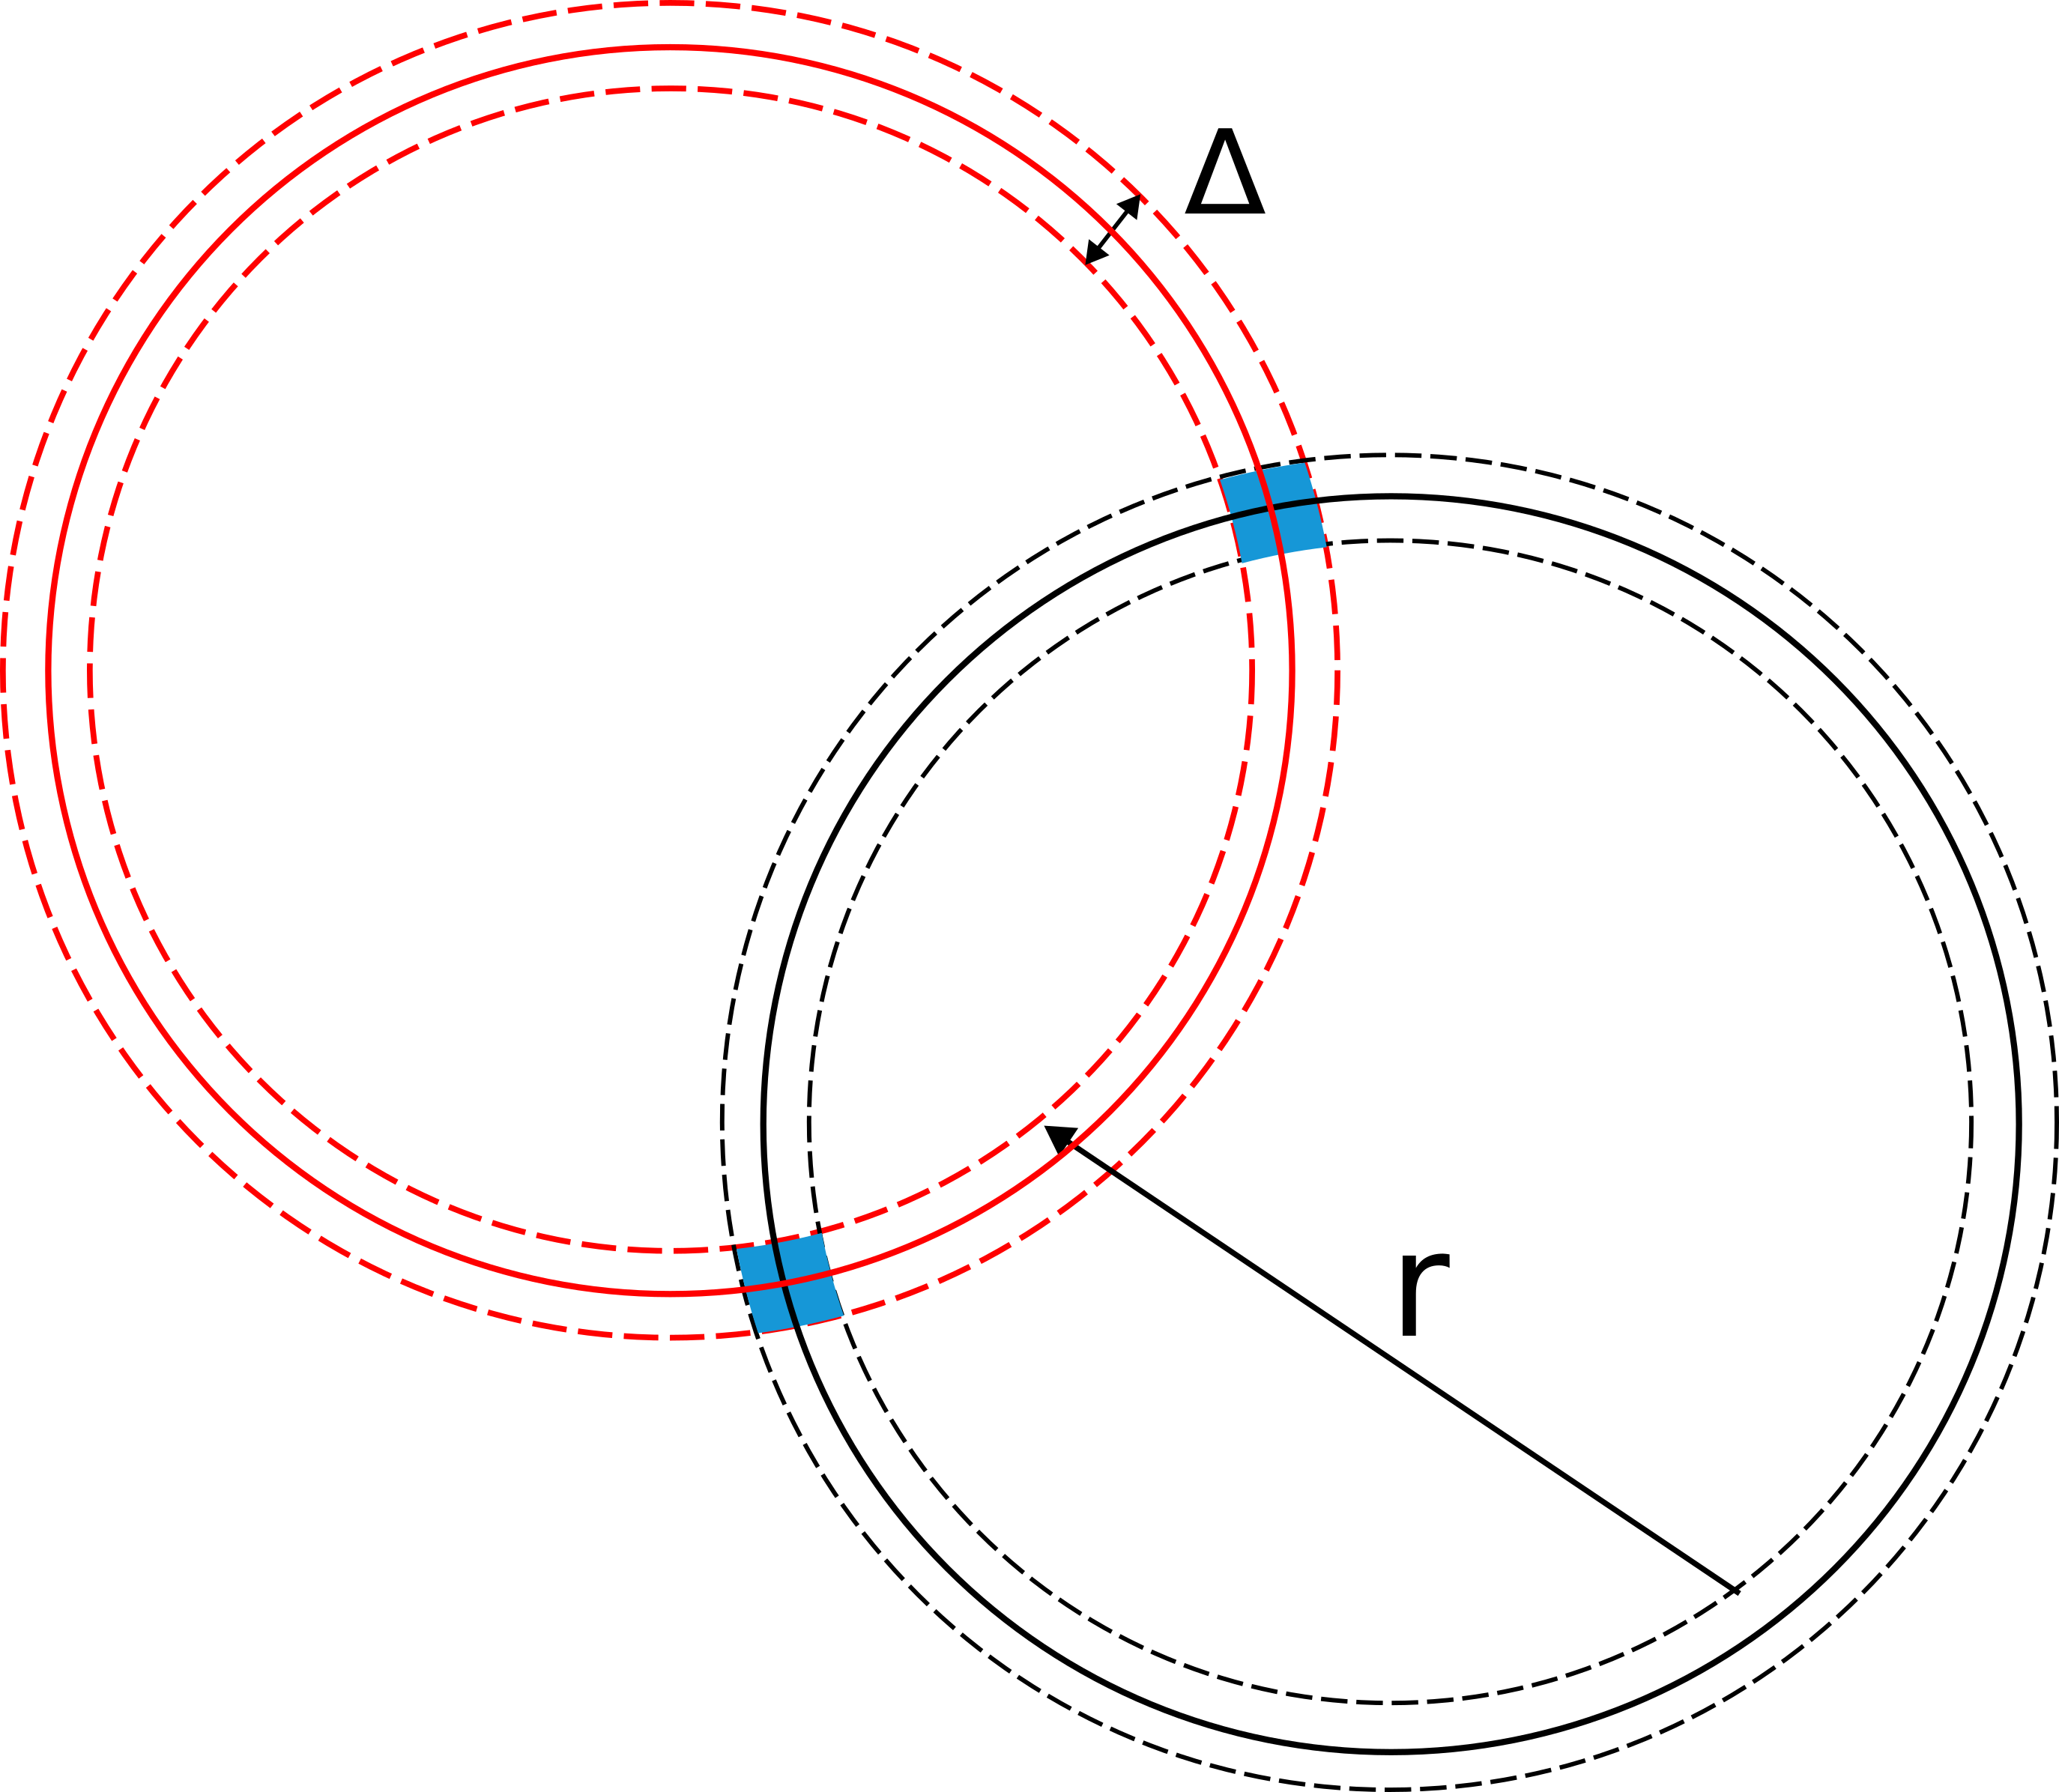
\includegraphics[width=0.8\linewidth]{images/Fss.png}
  \caption[]{Illustration of how $F_{ss}(\bm{r})$ is calculated. The interface
    between solid and void phases is a solid black curve. This interface
    translated by the vector $\bm{r}$ is show as a red solid curve. Support of
    $f_\Gamma(\bm{x}; \Delta)$ is a dashed ring. Shaded regions contribute to
    the surface-surface function.}
  \label{fig:Fss-explained}
\end{figure}
Let $S$ be some set in $\mathbb{R}^2$ which has a smooth boundary $\Gamma$ in
the sense that the boundary has a tangent line almost at every point. Now we
introduce a function $f_\Gamma(\bm{x}; \Delta)$:
\begin{equation*}
  f_\Gamma(\bm{x}; \Delta) = \left\{
  \begin{array}{ll}
    1/\Delta & \quad \rho(\bm{x}, \Gamma) < \Delta \\
    0 & \quad \text{otherwise}
  \end{array}
  \right.
\end{equation*}
Here $\rho(\bm{x}, \Gamma)$ means a closest distance from point $\bm{x}$ to the
boundary $\Gamma$.

\begin{figure}
  \centering
  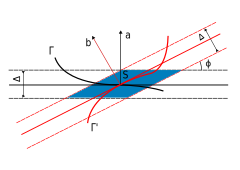
\includegraphics[width=0.8\linewidth]{images/fss-zoomed.png}
  \caption[]{Zoomed image of intersection between the interface $\Gamma$ and its
    translated version $\Gamma'$. $\phi$ is an angle between tangent lines to
    the interfaces. Surface of dashed area is $\frac{\Delta^2}{\sin \phi}$.}
  \label{fig:fss-zoomed}
\end{figure}
Now define a functional sequence $F_{ss}(\bm{x}; \Delta)$:
\begin{align*}
  F_{ss}(\bm{r}; \Delta) &= \int\int f_\Gamma(\bm{x}; \Delta) f_\Gamma(\bm{x}
  + \bm{r}; \Delta) dx dy \\
  &= \sum_{k=1}^N S_k/\Delta^2
\end{align*}
Here $N$ is a number of intersections of $\Gamma$ with itself translated by a
vector $\bm{r}$ and $S_k$ is a surface of each such intersection (see
\cref{fig:Fss-explained}).
When $\Delta$ tends to zero, the boundary at the point of intersection can
be replaced with a tangent line at the point of intersection
(\cref{fig:fss-zoomed}). We get an expression for a surface of
intersection: $S_k = \frac{\Delta^2}{\sin \phi_k}$ where $\phi_k$ is an
acute angle between tangent lines. Hence, we get the following equation:
\begin{equation}
  F_{ss}(\bm{r}) = \lim_{\Delta \to 0} F_{ss}(\bm{r}; \Delta) =
  \sum_{k=1}^N \frac{1}{\sin \phi_k} \label{eq:fss-2d}
\end{equation}
It's easy to show that
$\lim_{\Delta \to 0} f_\Gamma(\bm{x}; \Delta) = |\nabla \chi_A(\bm{x})|$
and therefore \cref{eq:fss-2d} and \cref{eq:fss} define the same function.

\subsection{Dual numbers and automatic differentiation}
\label{sec:dual}
A ring of dual numbers $D$ is a set of pairs of real numbers $(x, y)$ with two
binary operations: $+$ (addition) and $\cdot$ (multiplication) where
multiplication works according to the following law:
\begin{equation*}
  (x_1, y_1)\cdot(x_2, y_2) = (x_1x_2, x_1y_2 + y_1x_2)
\end{equation*}
It's easy to see that $D$ is commutative.

It's useful to introduce an imaginary unit $\varepsilon$ and write a dual number
$(x, y)$ as $x + y\varepsilon$. As you can see from multiplication law,
$1\cdot \varepsilon = \varepsilon$ and $\varepsilon^2 = 0$, hence $D$ is not an
integral domain and division is not defined for all dual numbers with exception
of $0$. Namely it's defined only if divisor has non-zero real part:
\begin{align*}
  \frac{a+b\varepsilon}{c+d\varepsilon} &=
  \frac{(a+b\varepsilon)(c-d\varepsilon)}{(c+d\varepsilon)(c-d\varepsilon)} \\
  &= \frac{ac-ad\varepsilon+bc\varepsilon}{c^2} \\
  &= \frac{a}{c} + \frac{bc-ad}{c^2}\varepsilon
\end{align*}

Power function $(a + b\varepsilon)^n$ where $n \in \mathbb{N}$ can be defined
using binomial formula and keeping in mind that $\varepsilon^n = 0$ if $n>1$:
\begin{equation*}
  (a + b\varepsilon)^n = \sum_{k=0}^n \binom{n}{k} a^k (b\varepsilon)^{n-k} =
  a^n + n a^{n-1} b \varepsilon
\end{equation*}
This formula can be extended on $n \in \mathbb{Q}$ as well.

Elementary functions can be extended to dual numbers using Taylor series. For
example, the exponent function is extended as:
\begin{align*}
  e^{a + b\varepsilon} &= \sum_{k=0}^{\infty}\frac{(a + b\varepsilon)^k}{k!} \\
  &= \sum_{k=0}^{\infty} \frac{a^k + bka^{k-1}\varepsilon}{k!} \\
  &= \sum_{k=0}^{\infty} \frac{a^k}{k!} + b\varepsilon \sum_{k=1}^{\infty}
  \frac{a^{k-1}}{(k-1)!} \\
  &= e^a + e^ab\varepsilon
\end{align*}

Here are some basic rules for working with dual numbers (some of which we have
already described):
\begin{itemize}
\item $(a + b\varepsilon) + (c + d\varepsilon) = (a + c) + (b + d)\varepsilon$
\item $(a + b\varepsilon) (c + d\varepsilon) = ac + (ad + bc)\varepsilon$
\item $\frac{a + b\varepsilon}{c + d\varepsilon} = \frac{a}{c} + \frac{bc - ad}{c^2}$
\item $\exp(a + b\varepsilon) = \exp(a) + b\varepsilon\exp(a)$
\item $\sin(a + b\varepsilon) = \sin(a) + b\varepsilon\cos(a)$
\item $\cos(a + b\varepsilon) = \cos(a) - b\varepsilon\sin(a)$
\item $\tan(a + b\varepsilon) = \tan(a) - \frac{b}{cos^2(a)}\varepsilon$
\end{itemize}

It's easy to see, that there is a connection between dual numbers and
differentiation. Indeed, if functions $f(x)$ and $g(x)$
are differentiable at the point $a$ and $h(x) = f(x)g(x)$ is their product then
$h(a + b\varepsilon) = h(a) + b\varepsilon(f'(a)g(a) + f(a)g'(a))$.
If $h(x) = f(x)/g(x)$ and $g(a) \ne 0$ then
$h(a + b\varepsilon) = h(a) + b\varepsilon\frac{f'(a)g(a) - f(a)g'(a)}{f^2(a)}$.
More generally, we can see that $f(a + b\varepsilon) = f(a) + bf'(a)\varepsilon$.

So, using dual numbers we can compute two values at once: one of the function at
the point $x = a$ and the other of its derivative at this point:
$f(a + \varepsilon) = f(a) + \varepsilon f'(a)$. Also we can compute a partial
derivative of a multivariate function. For example:
\begin{align*}
  \frac{\partial}{\partial x} f(x, y) \vert_{x = a, y = b} &= f(a + \varepsilon,
  b) \\
  \frac{\partial}{\partial y} f(x, y) \vert_{x = a, y = b} &= f(a, b +
  \varepsilon)
\end{align*}

\subsection{Surface-surface function for two-dimensional sets with smooth boundary}
\label{sec:cool-algo}
Here we examine two-dimensional sets with smooth boundary described in
\cref{sec:fss-2d} more closely. Suppose a set $S$ is defined as
$S = \left\{ (x, y) \ | \quad f(x, y) \le T \right\}$ where $f(x, y)$ is some function
differentiable at points where $f(x, y) = T$ and $T$ is some threshold. Let's
calculate surface-surface function for this set at a point $(a, b)$. We find all
intersections between a boundary $\Gamma$ and its translated version by solving a
system of equations
\begin{equation*}
  \left\{
  \begin{array}{l}
    f(x, y) = T \\
    f(x-a, y-b) = T    
  \end{array}
  \right.
\end{equation*}
which can be replaced by one equation
\begin{equation}
  (f(x, y) - T)^2 + (f(x-a, y-b) - T)^2 = 0 \label{eq:inter}
\end{equation}
We denote a set of solutions of this equation as $X$. For every $\bm{x}_i \in X$
we find an angle $\phi_i$ between a normal to the boundary and a normal to
the translated boundary as
\begin{equation}
  \cos \phi_i = \frac{(\nabla f(x,y) \vert_{\bm{x}_i}, \nabla f(x-a,y-b)
    \vert_{\bm{x}_i})}{|\nabla f(x,y) \vert_{\bm{x}_i}| |\nabla f(x-a,y-b)
    \vert_{\bm{x}_i}|} \label{eq:angle}
\end{equation}
Here $(\cdot, \cdot)$ denotes a dot product. Gradient of $f$ at the point
$\bm{x_i}$ can be found using automatic differentiation and dual numbers
described in \cref{sec:dual}. Note that acute angle between tangent lines equals
to acute angle between normals, therefore we can find correlation function
$F_{ss}(a, b)$ using the following formula:
\begin{equation}
  F_{ss}(a, b) = \sum_i \frac{1}{\sqrt{1 - \cos^2 \phi_i}} \label{eq:fss-method}
\end{equation}

The algorithm of calculating $F_{ss}(a, b)$ is the following:
\begin{enumerate}
\item Find $X$ which is a set of soulutions of \cref{eq:inter}.
\item For all points in $X$ find cosines between normals to the boundaries using
  \cref{eq:angle}.
\item Calculate $F_{ss}(a, b)$ using \cref{eq:fss-method}.
\end{enumerate}

The set $X$ can be found by firstly evaluating $f(x, y)$ in some regular grid
searching for all points $(x_i, y_i)$ for which $|f(x_i, y_i) - T| < \epsilon$
and $|f(x_i - a, y_i - b) - T| < \epsilon$ for some positive $\epsilon$
and then using these points as starting points for some algorithm based on
gradient descent like ADAM to solve \cref{eq:inter}.

\section{Examples of two-dimensional sets with smooth boundary}
\label{seq:examples}
In this section we will provide few examples of sets for which the developed
precise algorithm is applicable and compare the surface-surface function
calculated with the fast algorithm (\cref{sec:algo}) with results of the new
algorithm. We will use the filter $H$ (\ref{eq:filter-3x3-2d}) for edge
detection along with a new filter $H'$ (\ref{eq:filter-5x5-2d}) described in
\cref{sec:improvement}.

\subsection{A square}
Let's define a function $f(x, y) = \max(|x|, |y|)$. A set $f(x, y) \le T$ is a
square with side $2T$. The function $f$ is differentiable at all points where
$f(x, y) = T$ with exception of points $(-T, -T)$, $(-T, T)$, $(T, -T)$ and
$(T, T)$. The surface-surface correlation function for a square is equal to:
\begin{equation*}
  F_{ss}(x, y) = \left\{
  \begin{array}{ll}
    2 & \quad \max(|x|, |y|) < T \ \text{and}\ x\ne0, y\ne0 \\
    0 & \quad \max(|x|, |y|) > T \\
    \text{undefined} & \quad \text{otherwise}
  \end{array}
  \right.
\end{equation*}
A graphical diagram depicting this case is shown on \cref{fig:fss-square}. In
this case the algorithm described in \cref{sec:algo} gives a correct result in
any point which is few pixels away from where $F_{ss}$ is undefined.
\begin{figure}
  \centering
  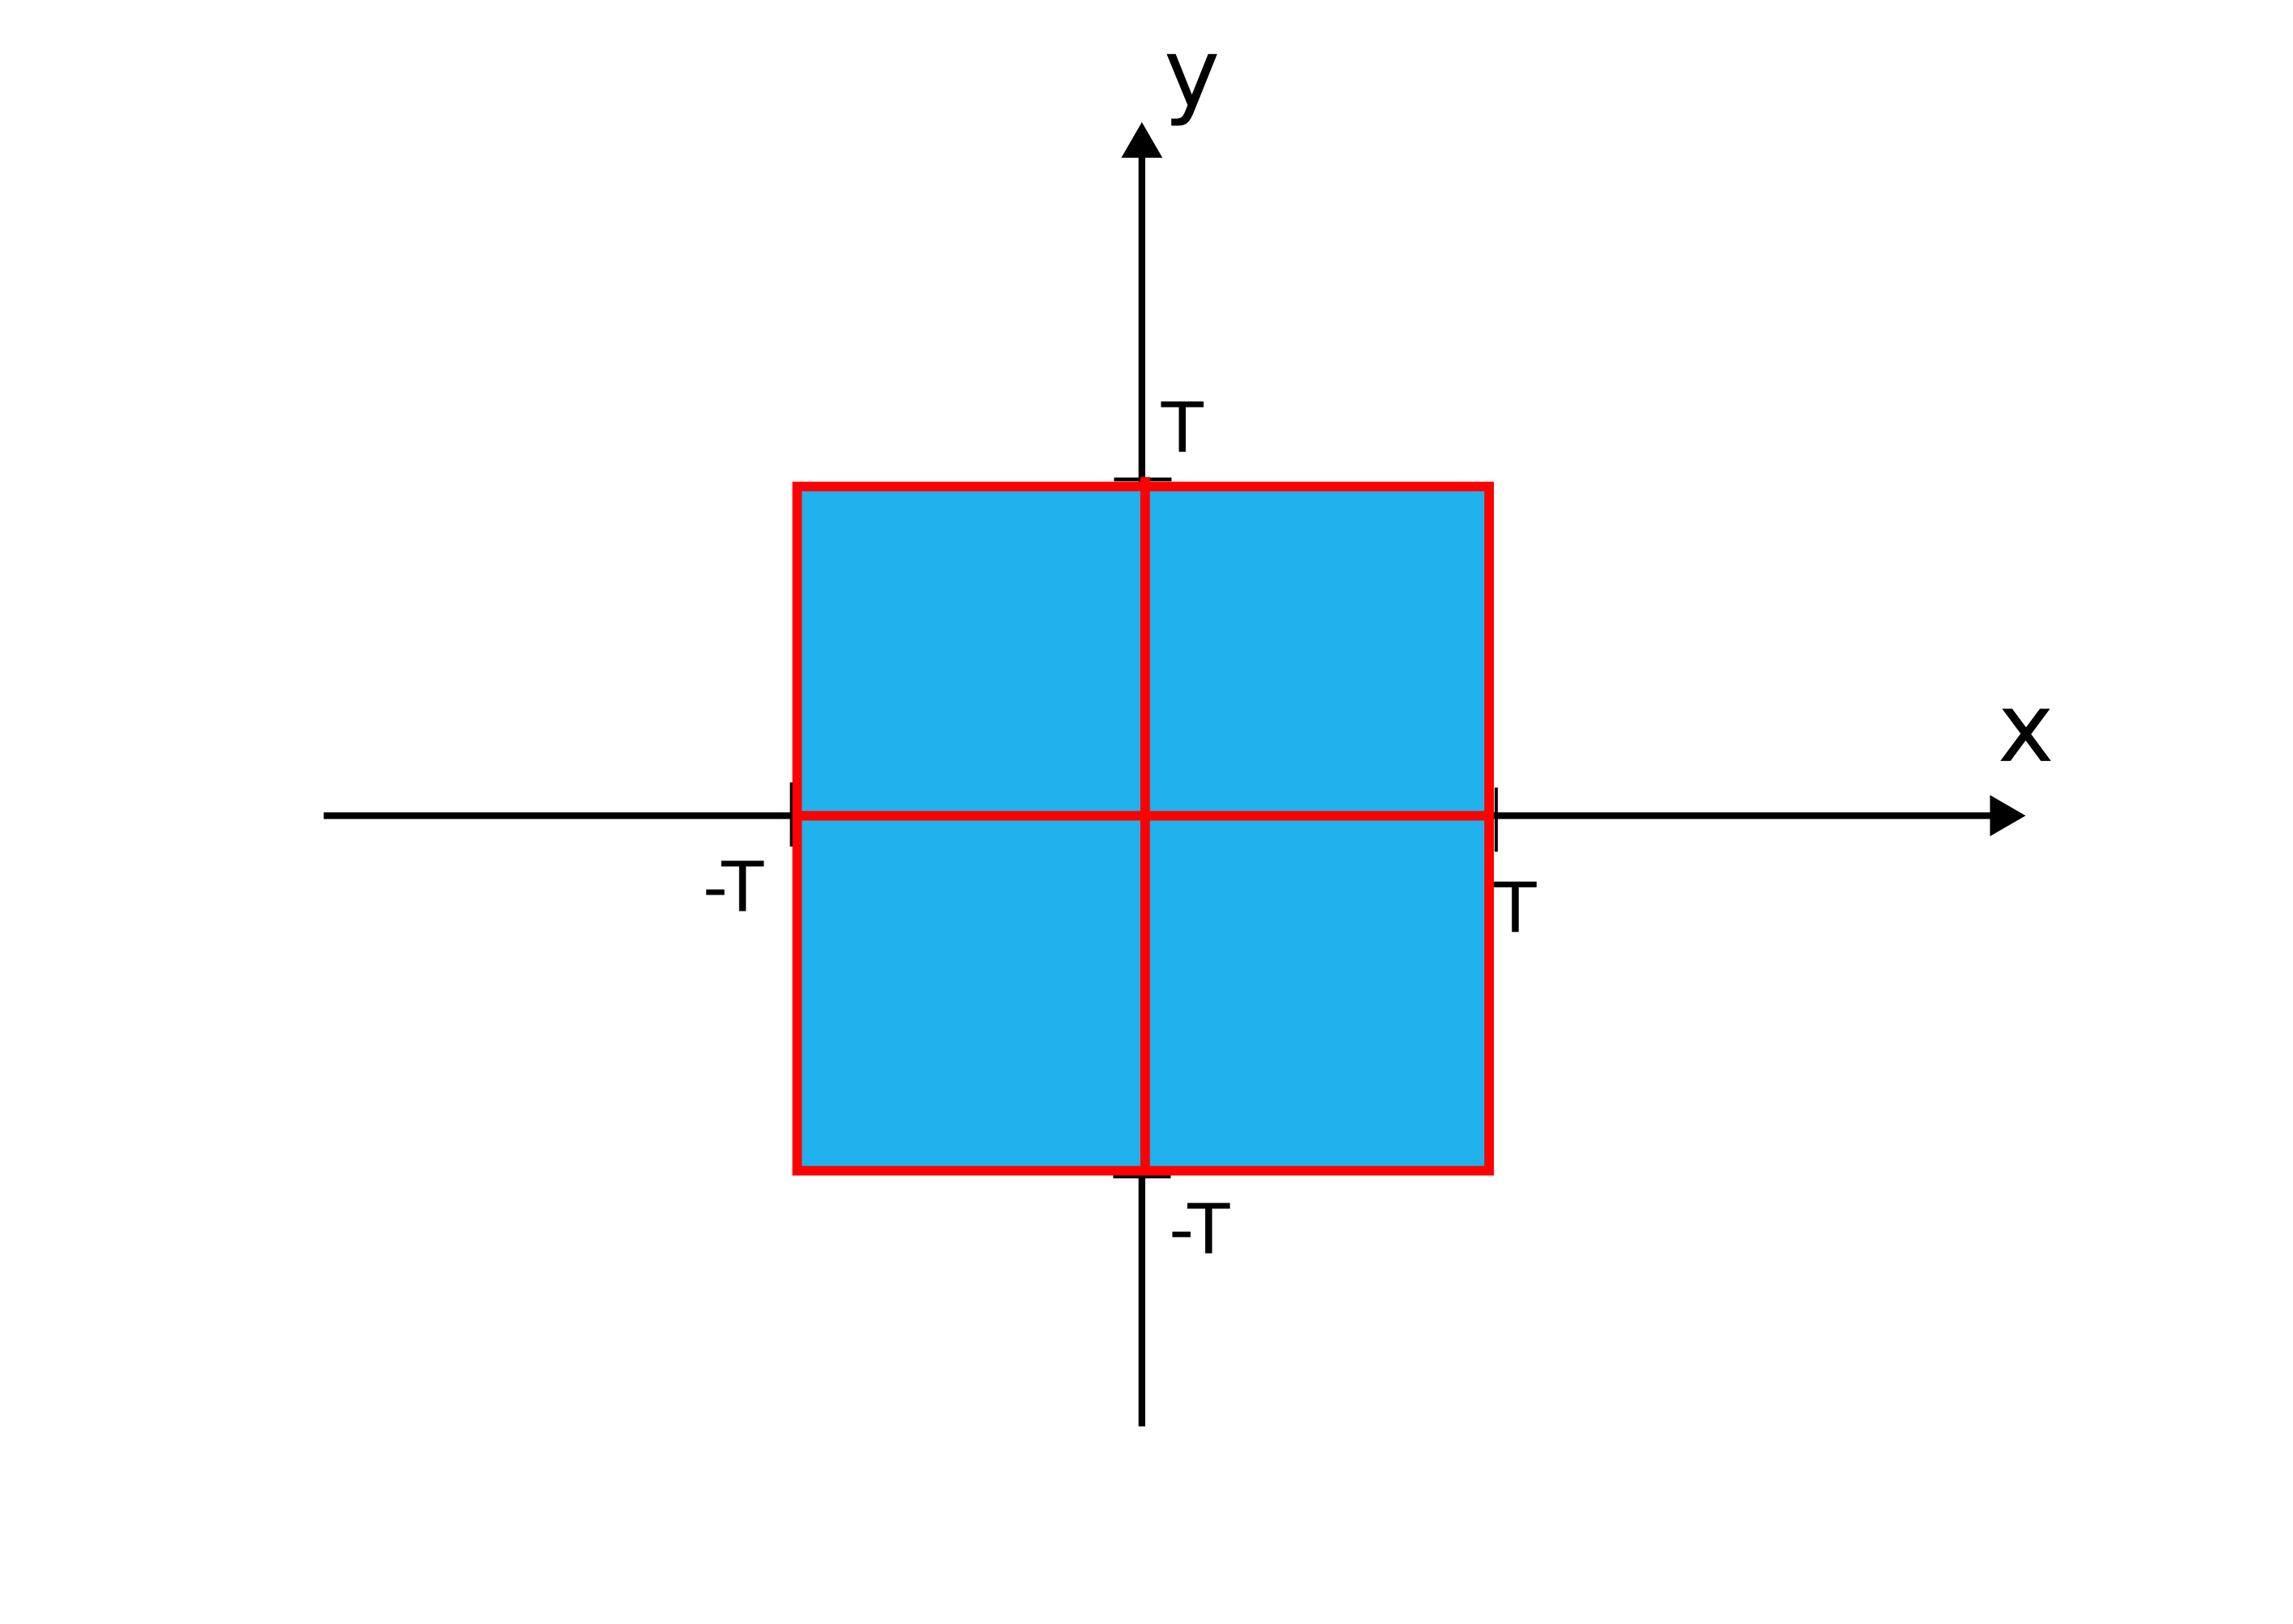
\includegraphics[width=0.8\linewidth]{images/fss-square.png}
  \caption[]{$F_{ss}$ function for a square with side $T$. The function is
    undefined along red segments. Its value is $2$ inside a shaded area and $0$
    outside.}
  \label{fig:fss-square}
\end{figure}

\subsection{A disk}
If we define $f(x, y) = x^2 + y^2$ then an inequation $f(x, y) \le R^2$ defines
a disk of radius $R$ with center at the origin. In this case $F_{ss}$ depends
only on distance $r$ from the origin:
\begin{equation*}
  F_{ss}(r) = \left\{
  \begin{array}{ll}
    \frac{4R^2}{r\sqrt{4R^2-r^2}} & \quad r < 2R \\
    0 & \quad \text{otherwise}
  \end{array}
  \right.
\end{equation*}
A comparison of the algorithm described in \cref{sec:algo} applied to images
with different resolution with a theory is shown on \cref{fig:fss-disk}.
\begin{figure*}[!pt]
  \centering
  \subfigure[$3\times 3$ kernel $H$]{
    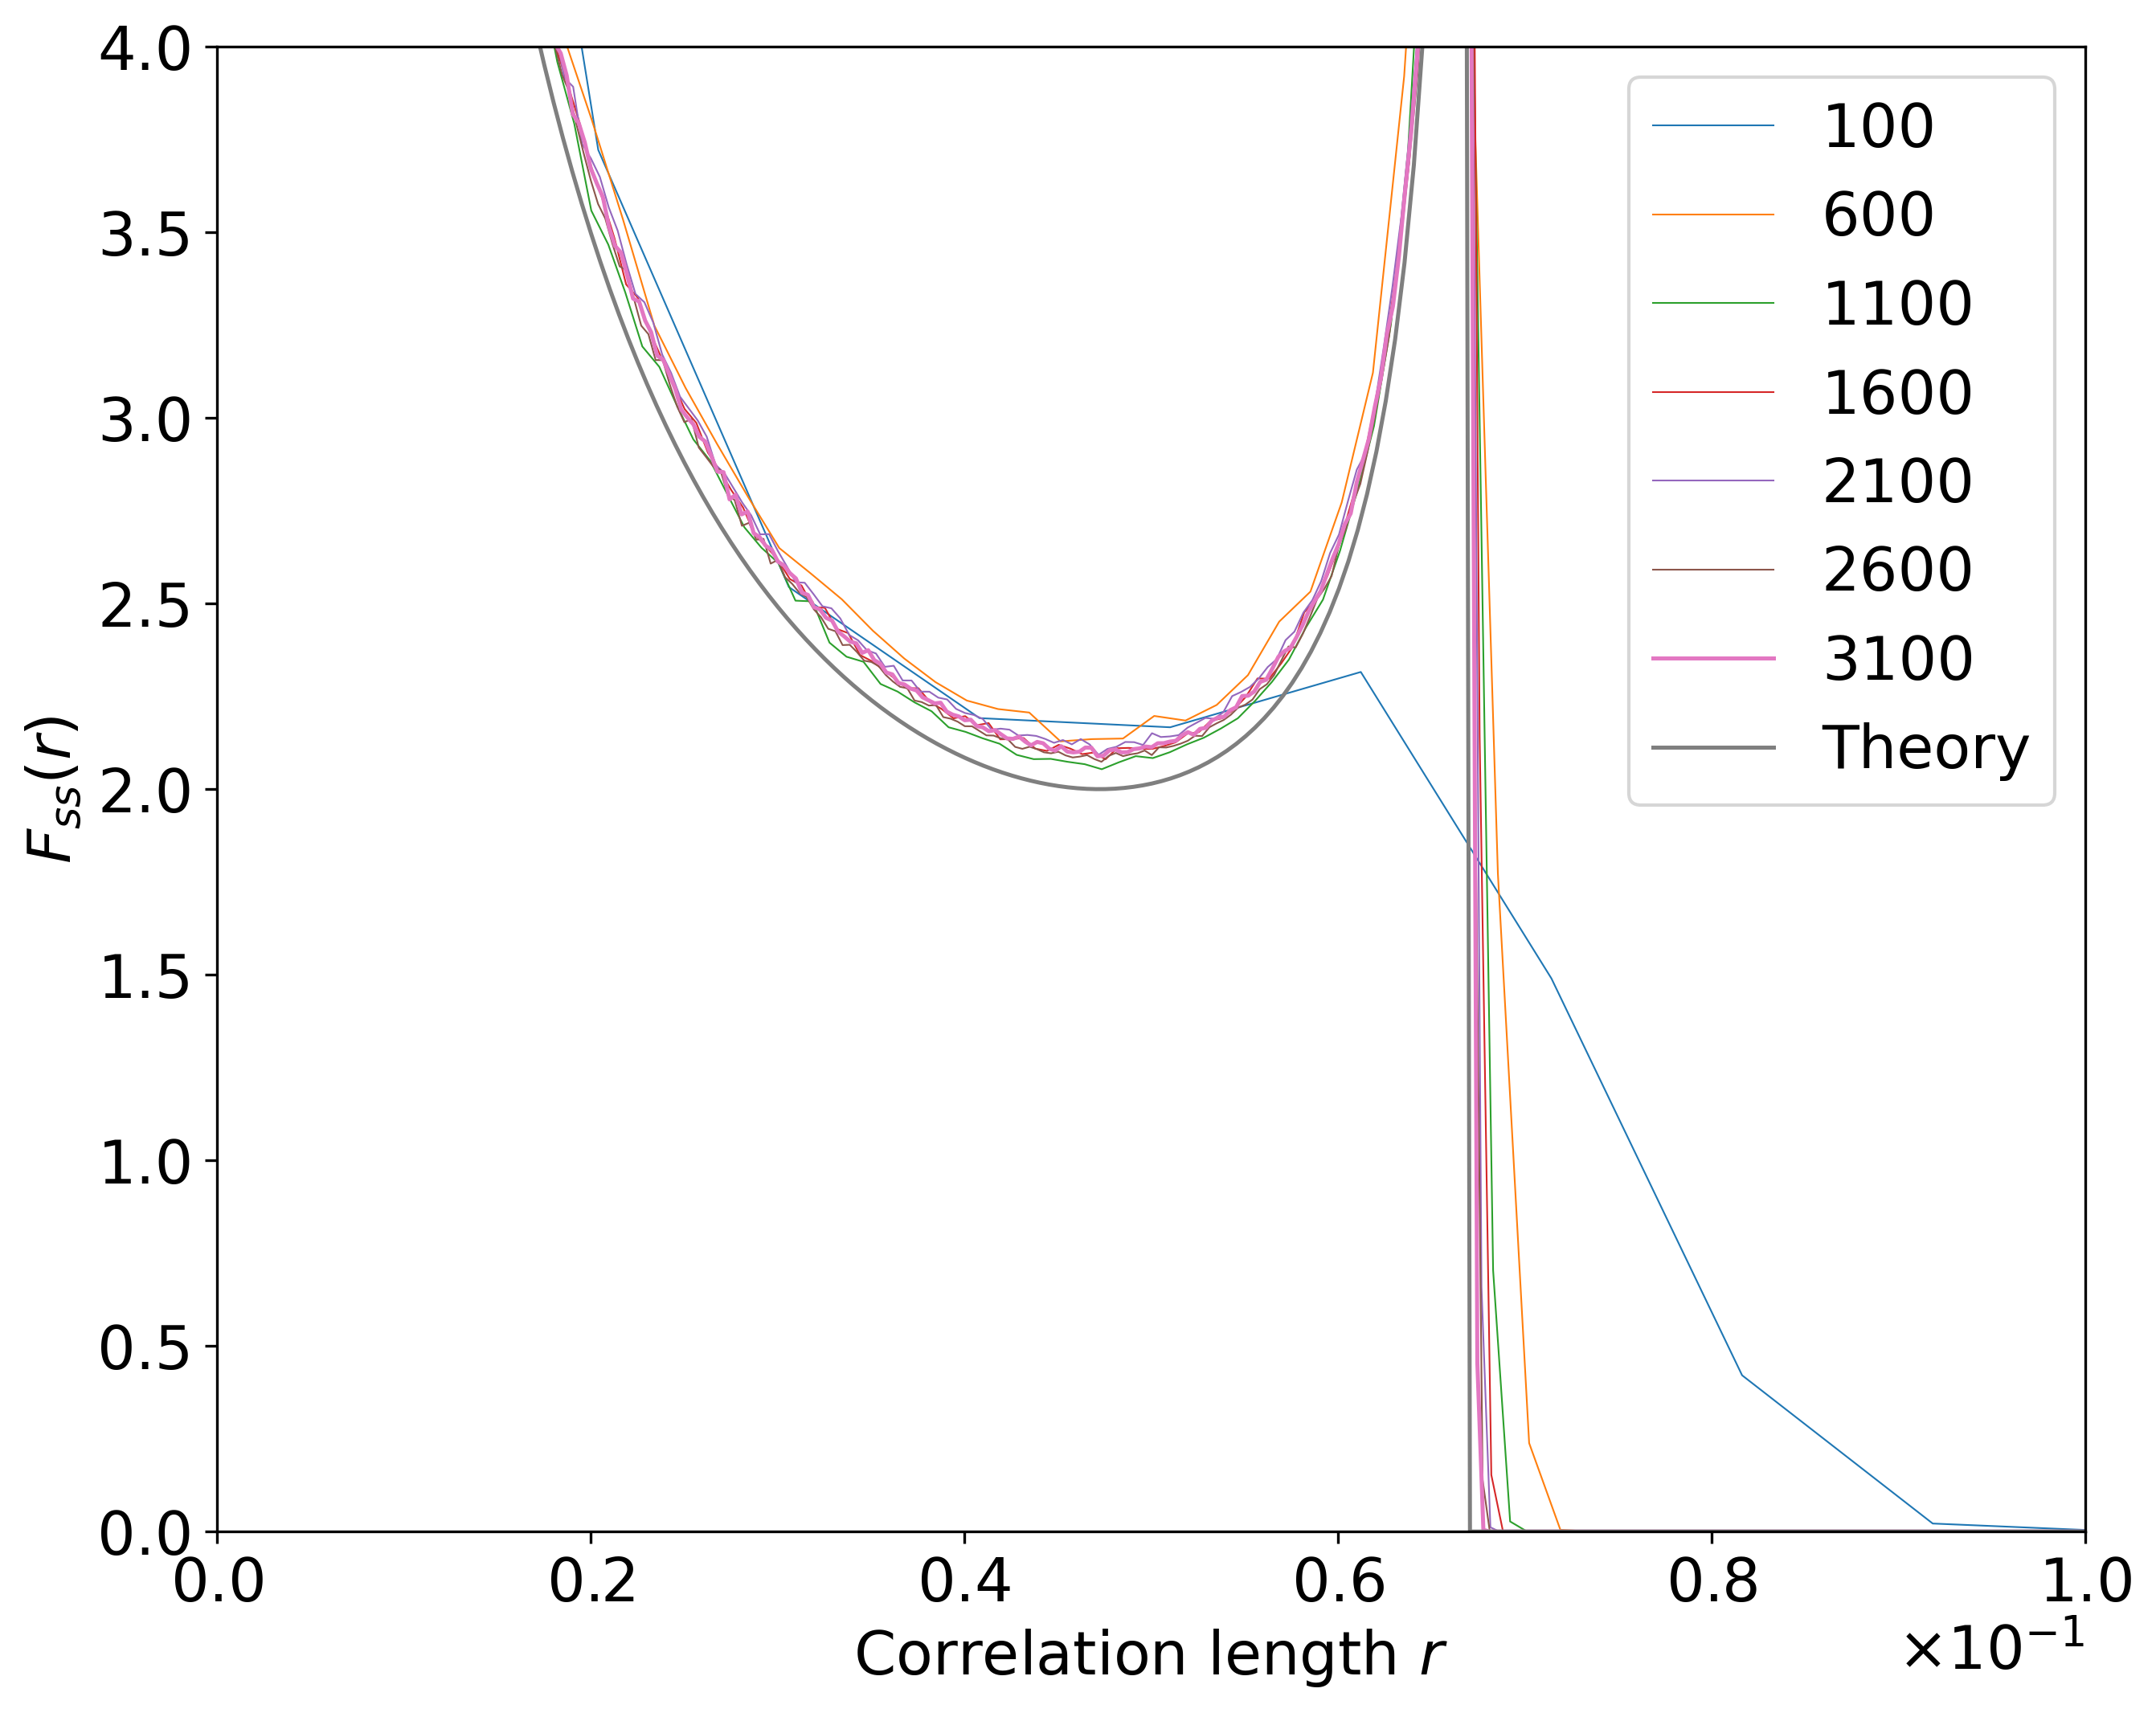
\includegraphics[width=0.45\linewidth]{images/fss-disk-3x3.png}
    \label{fig:fss-disk-3x3}}
  \hfill
  \subfigure[$5\times 5$ kernel $H'$]{
    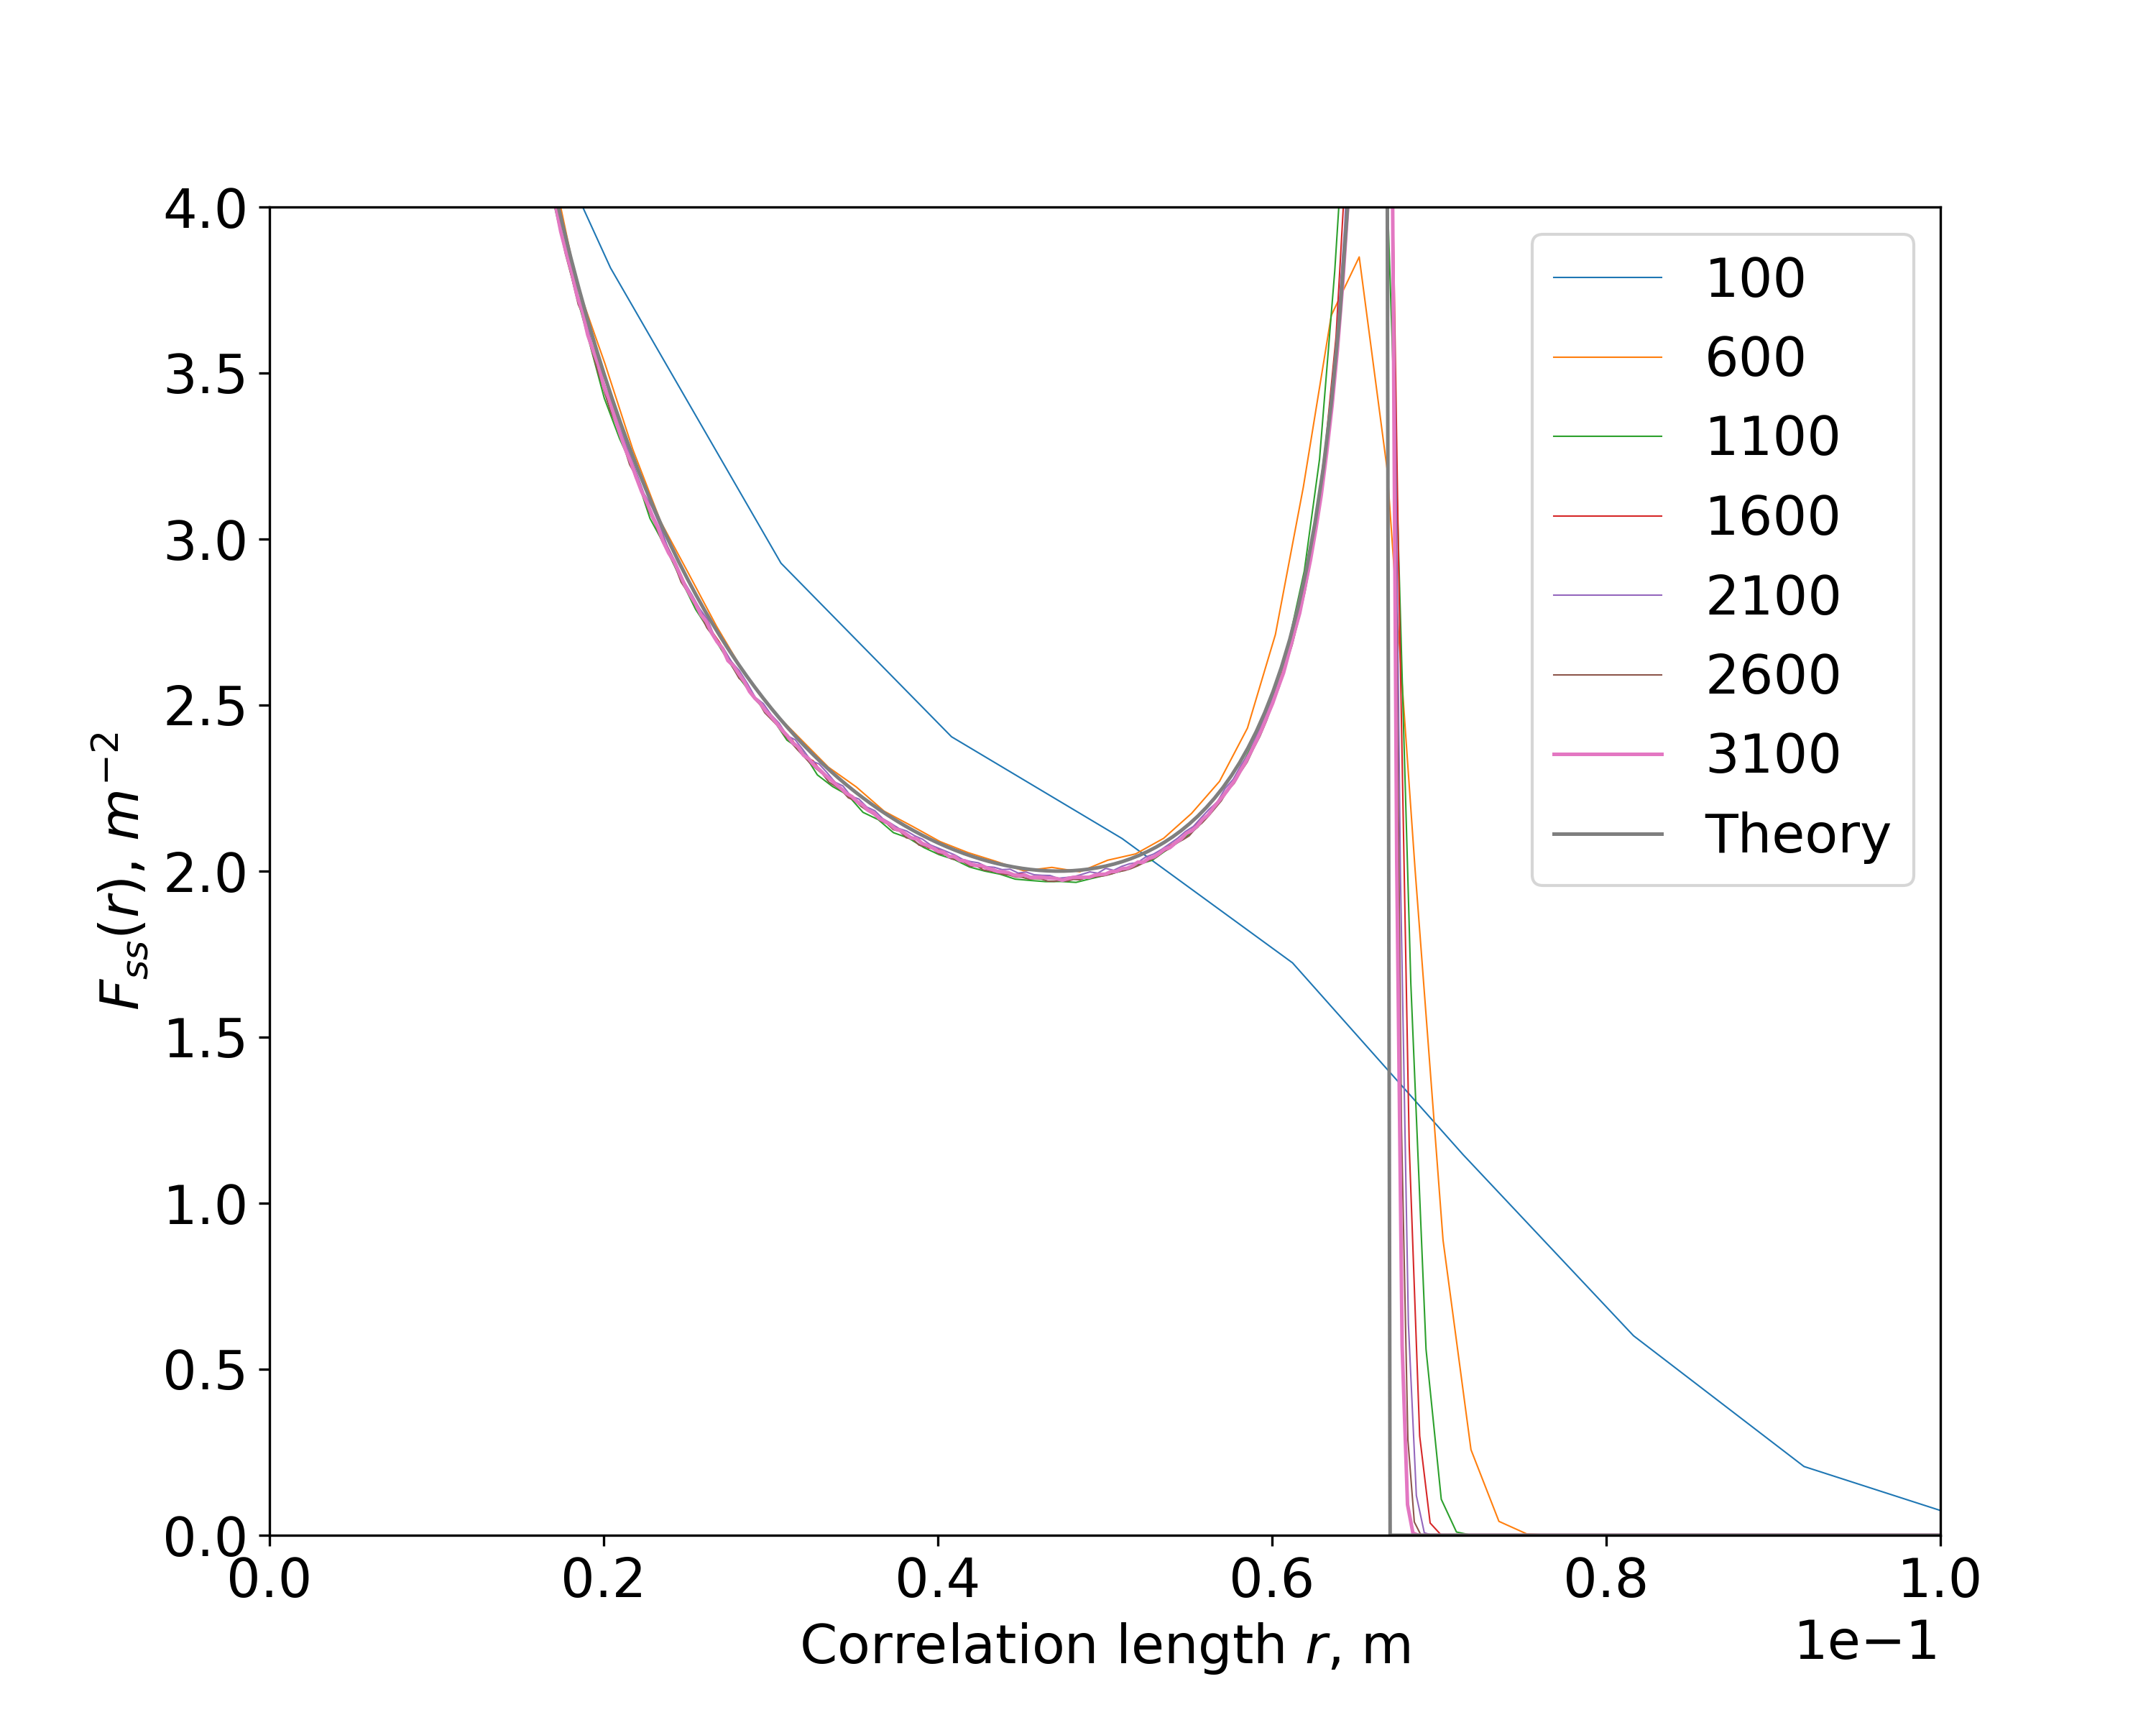
\includegraphics[width=0.45\linewidth]{images/fss-disk-5x5.png}
    \label{fig:fss-disk-5x5}}
  \caption[]{Plot of surface-surface function for a disk with radius
    $R = 0.0334$. Resolution of the image varies from $100\times 100$ pixels to
    $3100\times 3100$.}
  \label{fig:fss-disk}
\end{figure*}

\subsection{Gaussian mixture}
\label{sec:gauss}
\begin{figure}
  \centering
  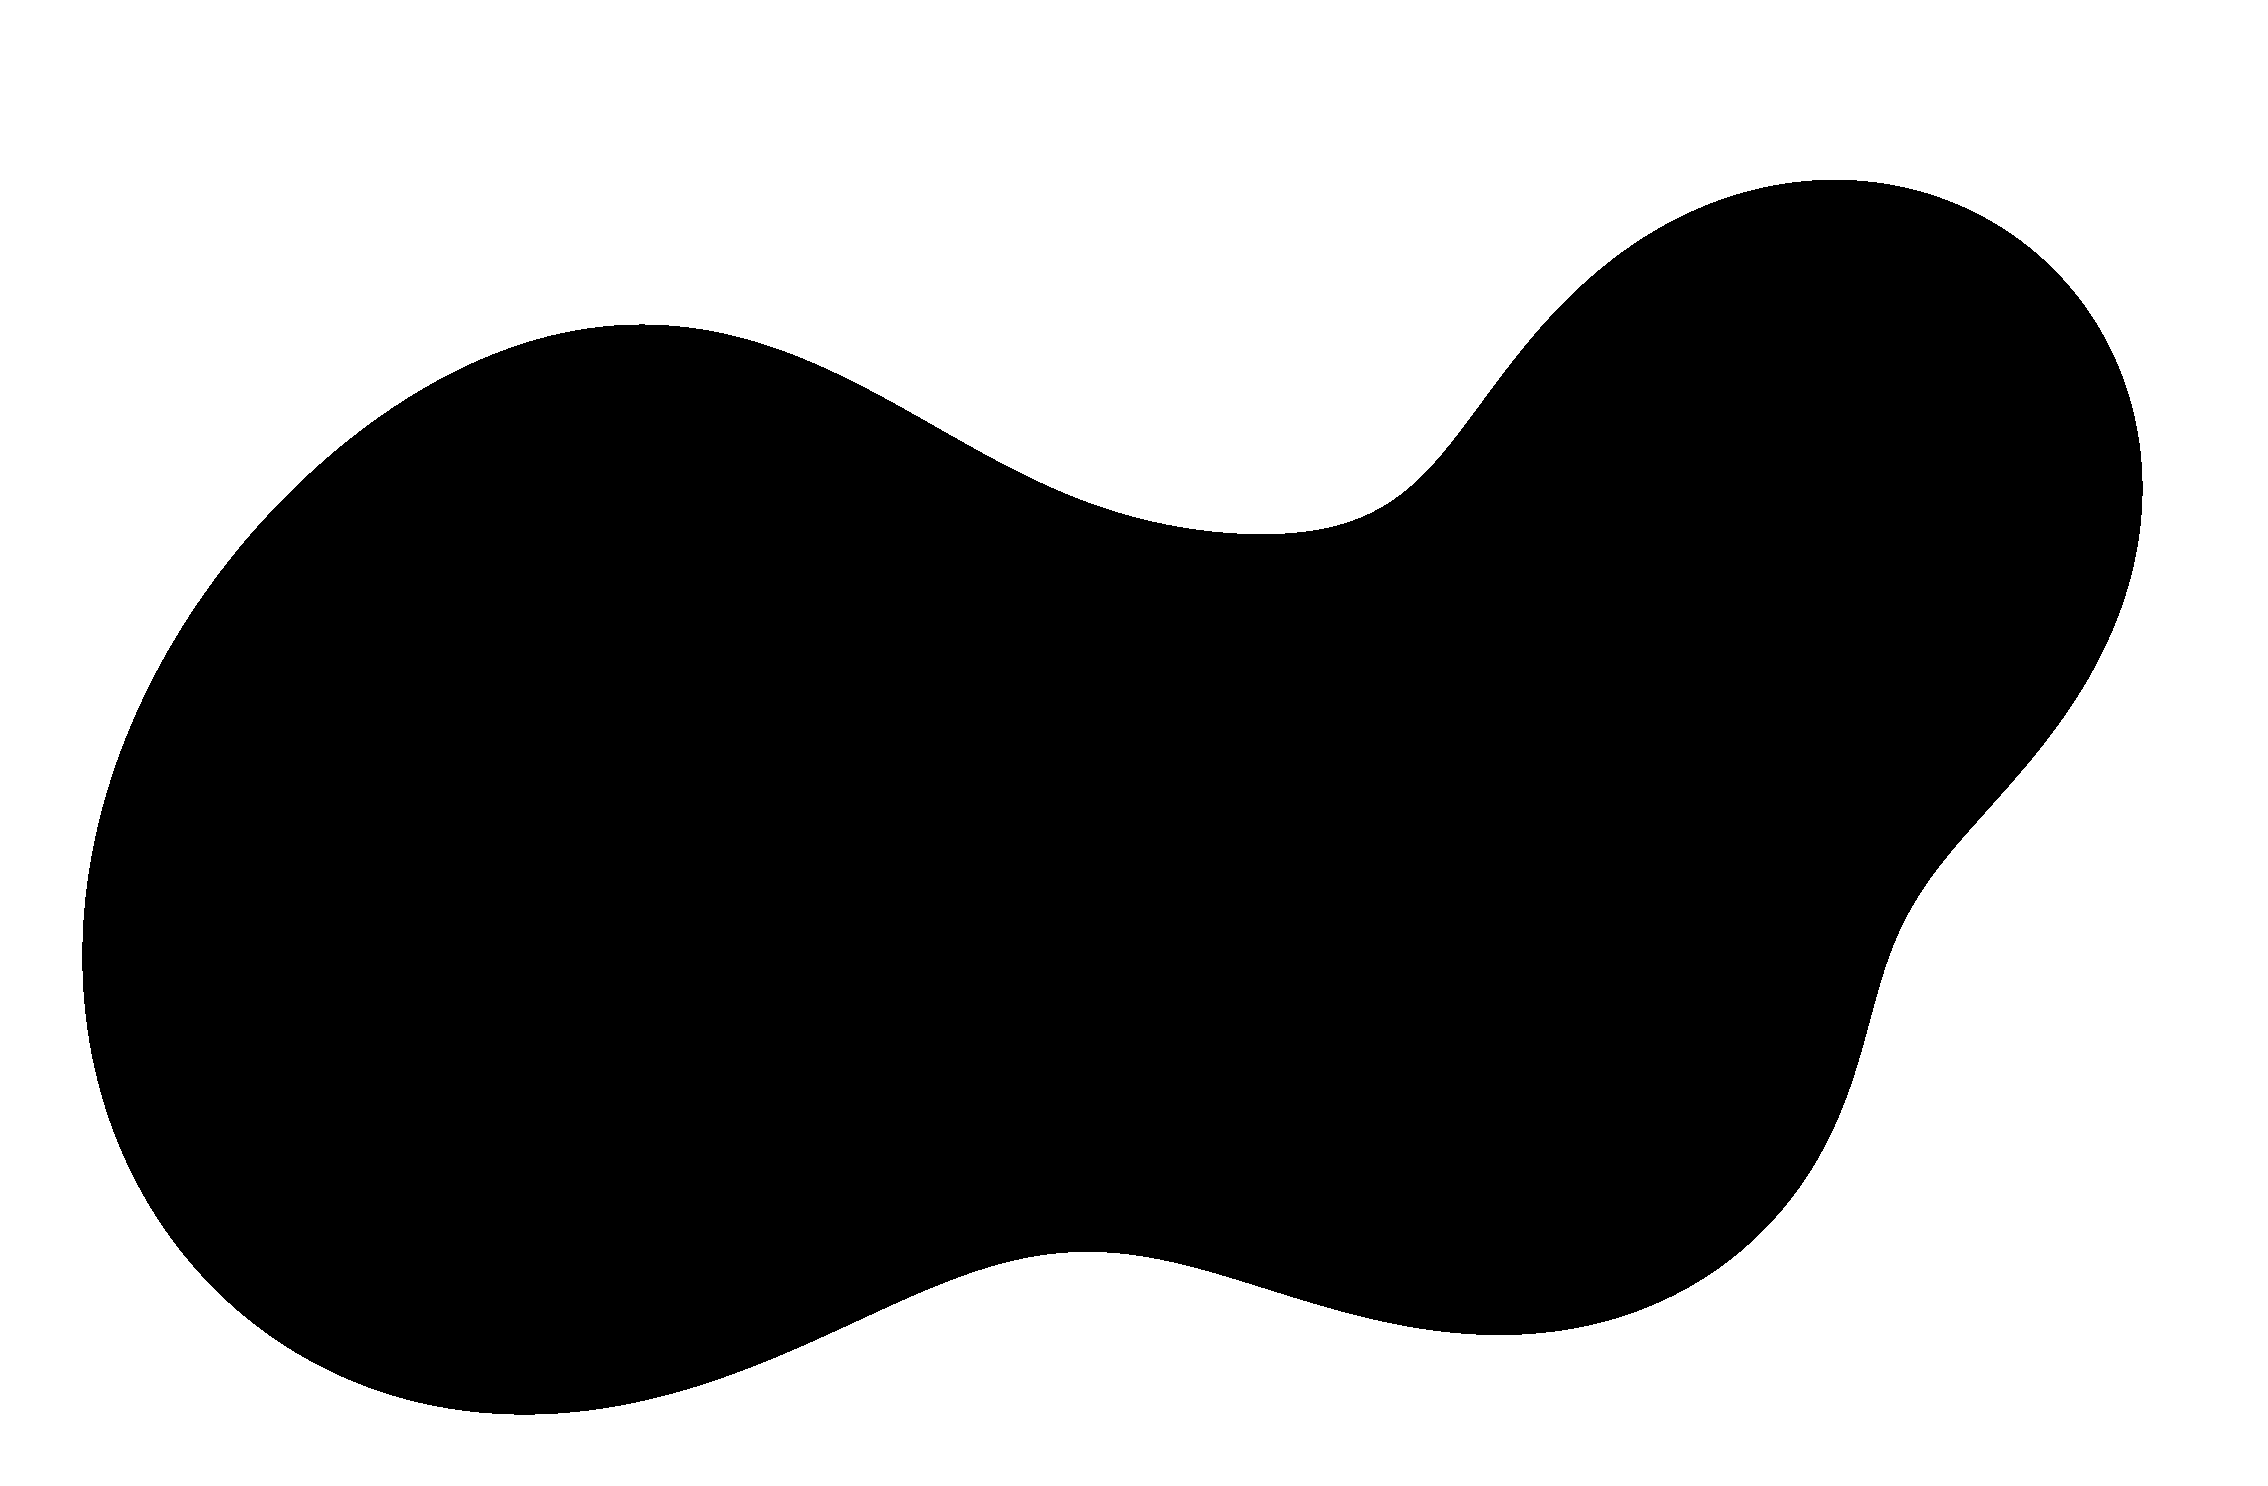
\includegraphics[width=0.8\linewidth, frame]{images/blob.png}
  \caption[]{An example of a ``blob'' generated by Gaussian mixture $f(x,y)$
    which consists of four Gaussian functions. White area is where
    $f(x,y) \le 3$.}
  \label{fig:blob}
\end{figure}
Take $N$ random values $a_i$, $b_i$ and $\sigma_i$. Let $f$ be
\begin{equation*}
  f(x,y) = \sum_{i=1}^N \frac{1}{\sigma_i} \exp(\frac{-(x-a_i)^2-(y-b_i)^2}{\sigma_i^2})
\end{equation*}
Inequality $f(x,y) \le T$ defines a ``blob'' like one which can be seen on
\cref{fig:blob}. We can use the algorithm developed in \cref{sec:cool-algo} to
compute precise values of $F_{ss}$ for this blob and compare them with values
obtained by using the fast algorithm in section \cref{sec:algo}. The result of
this comparison is on \cref{fig:fss-blob}.
\begin{figure*}[!pt]
  \centering
  \subfigure[$3\times 3$ kernel $H$]{
    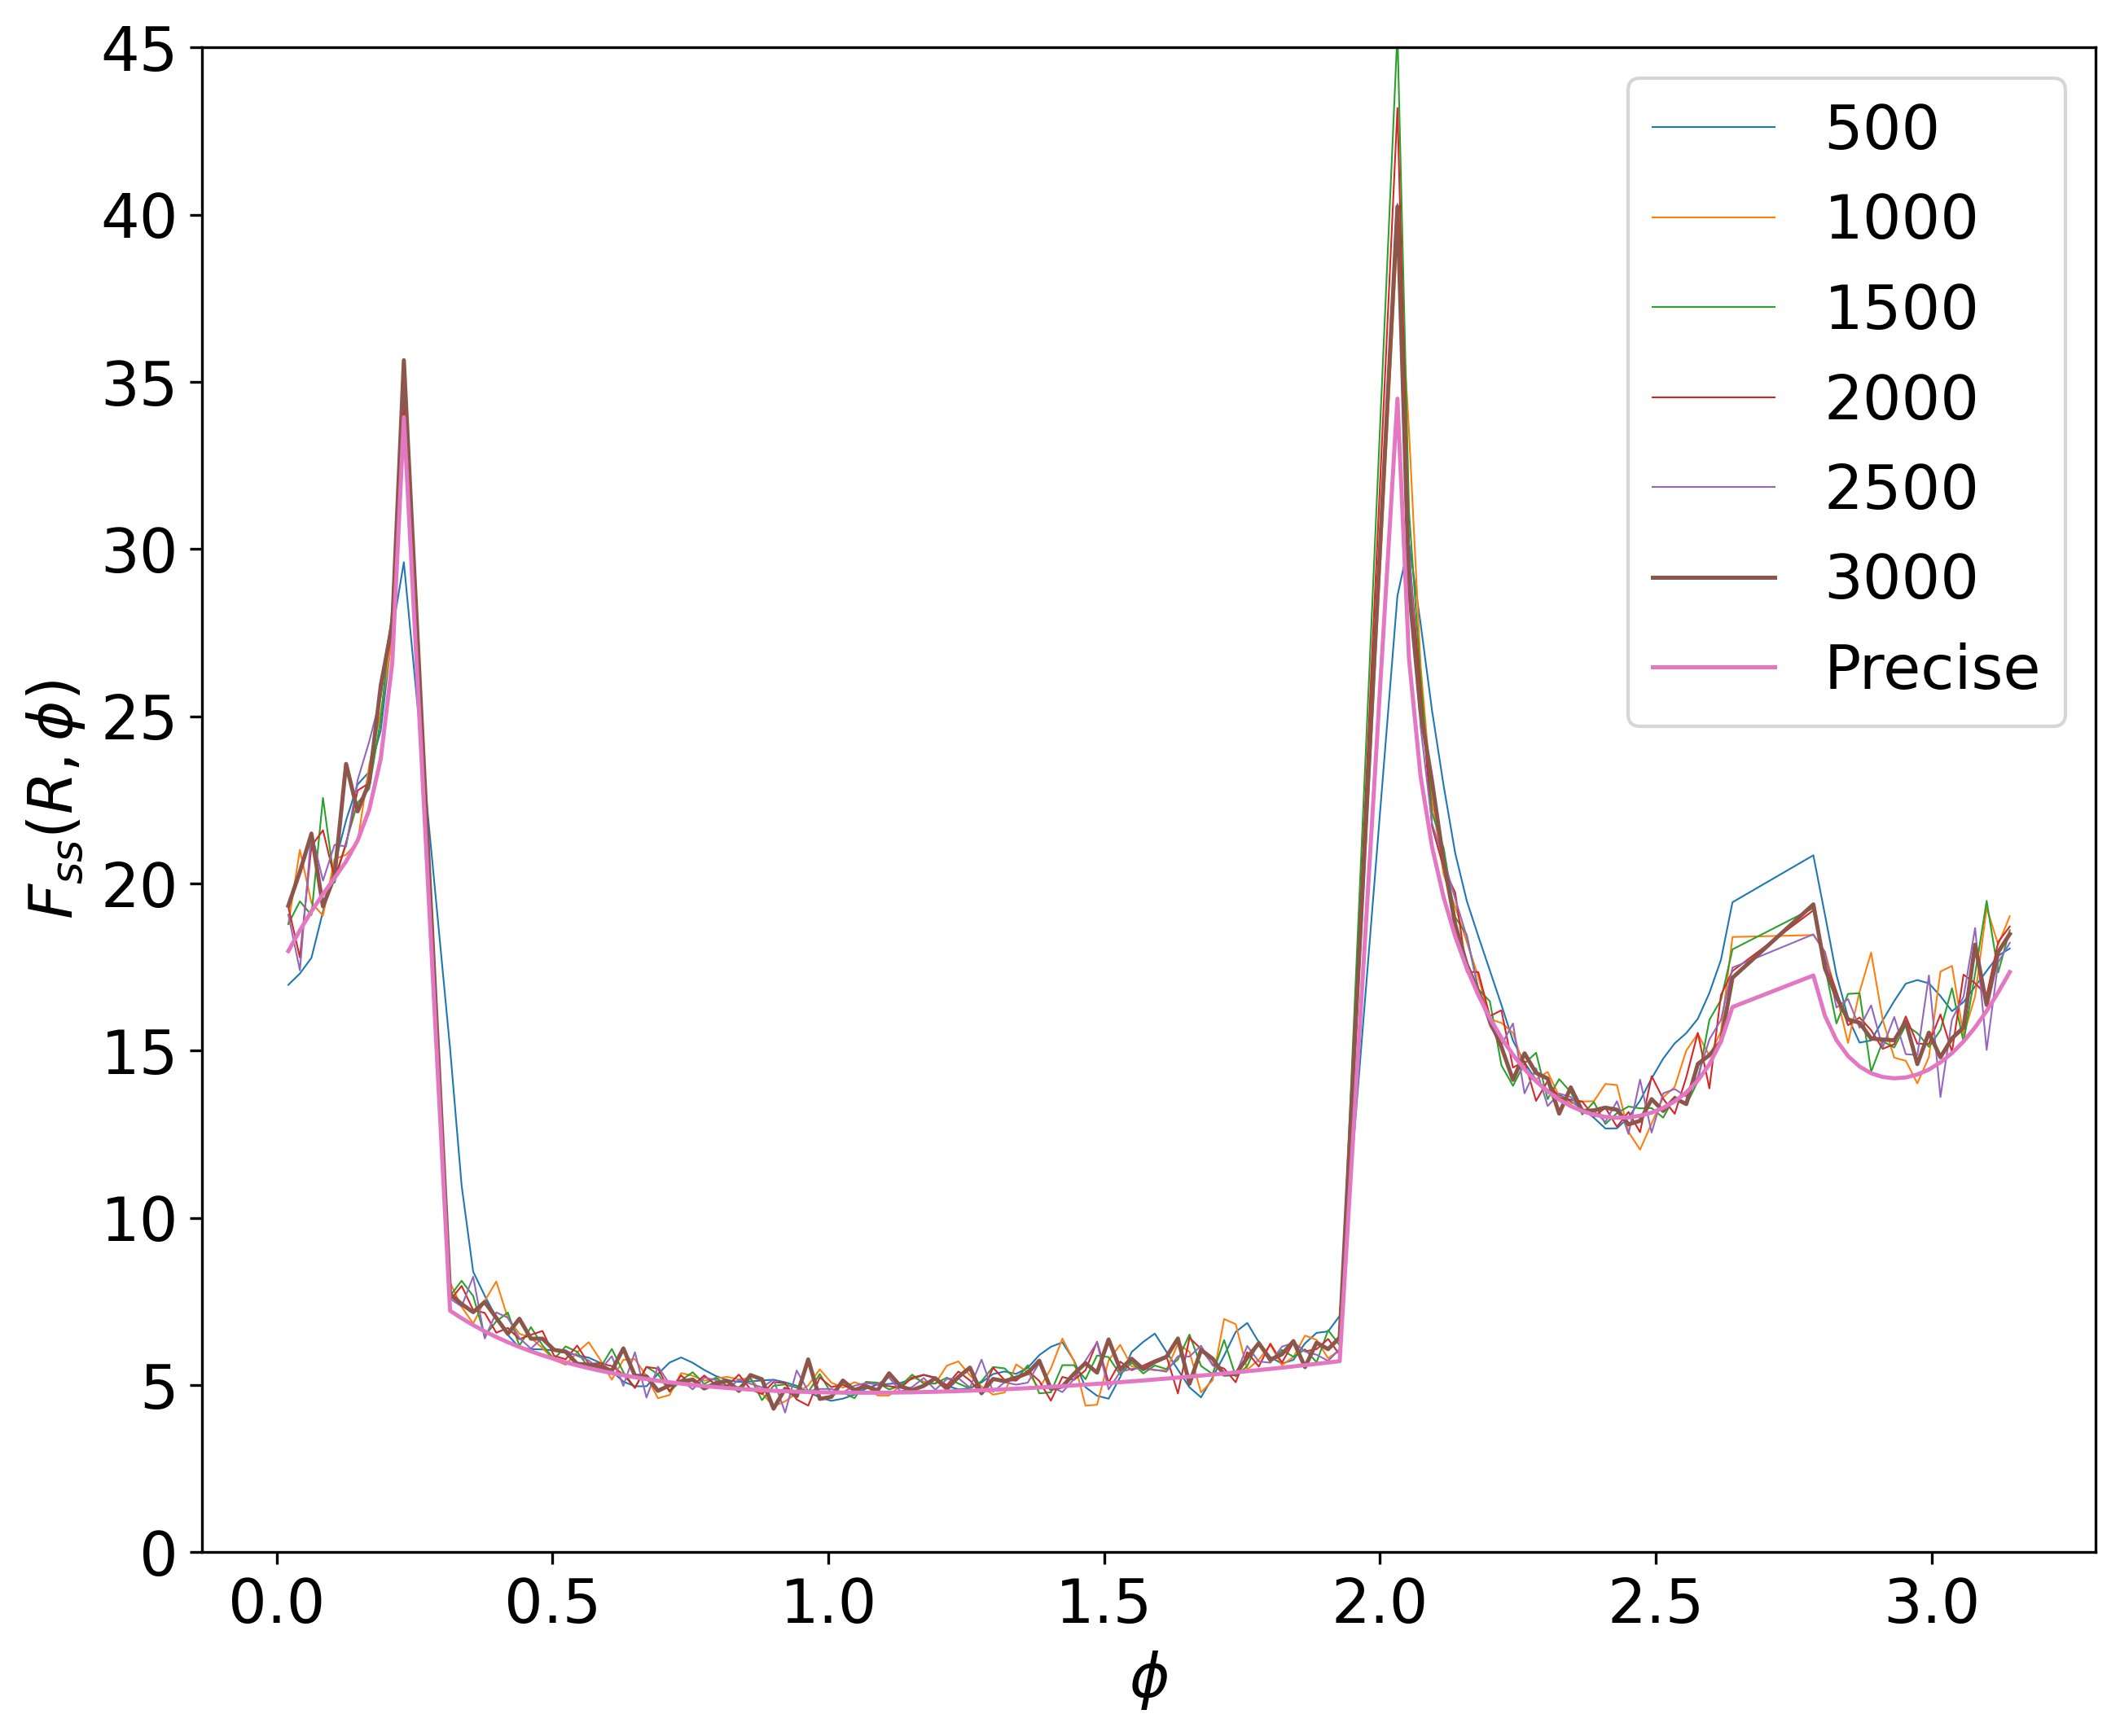
\includegraphics[width=0.45\linewidth]{images/fss-blob-3x3.png}
    \label{fig:fss-blob-3x3}}
  \hfill
  \subfigure[$5\times 5$ kernel $H'$]{
    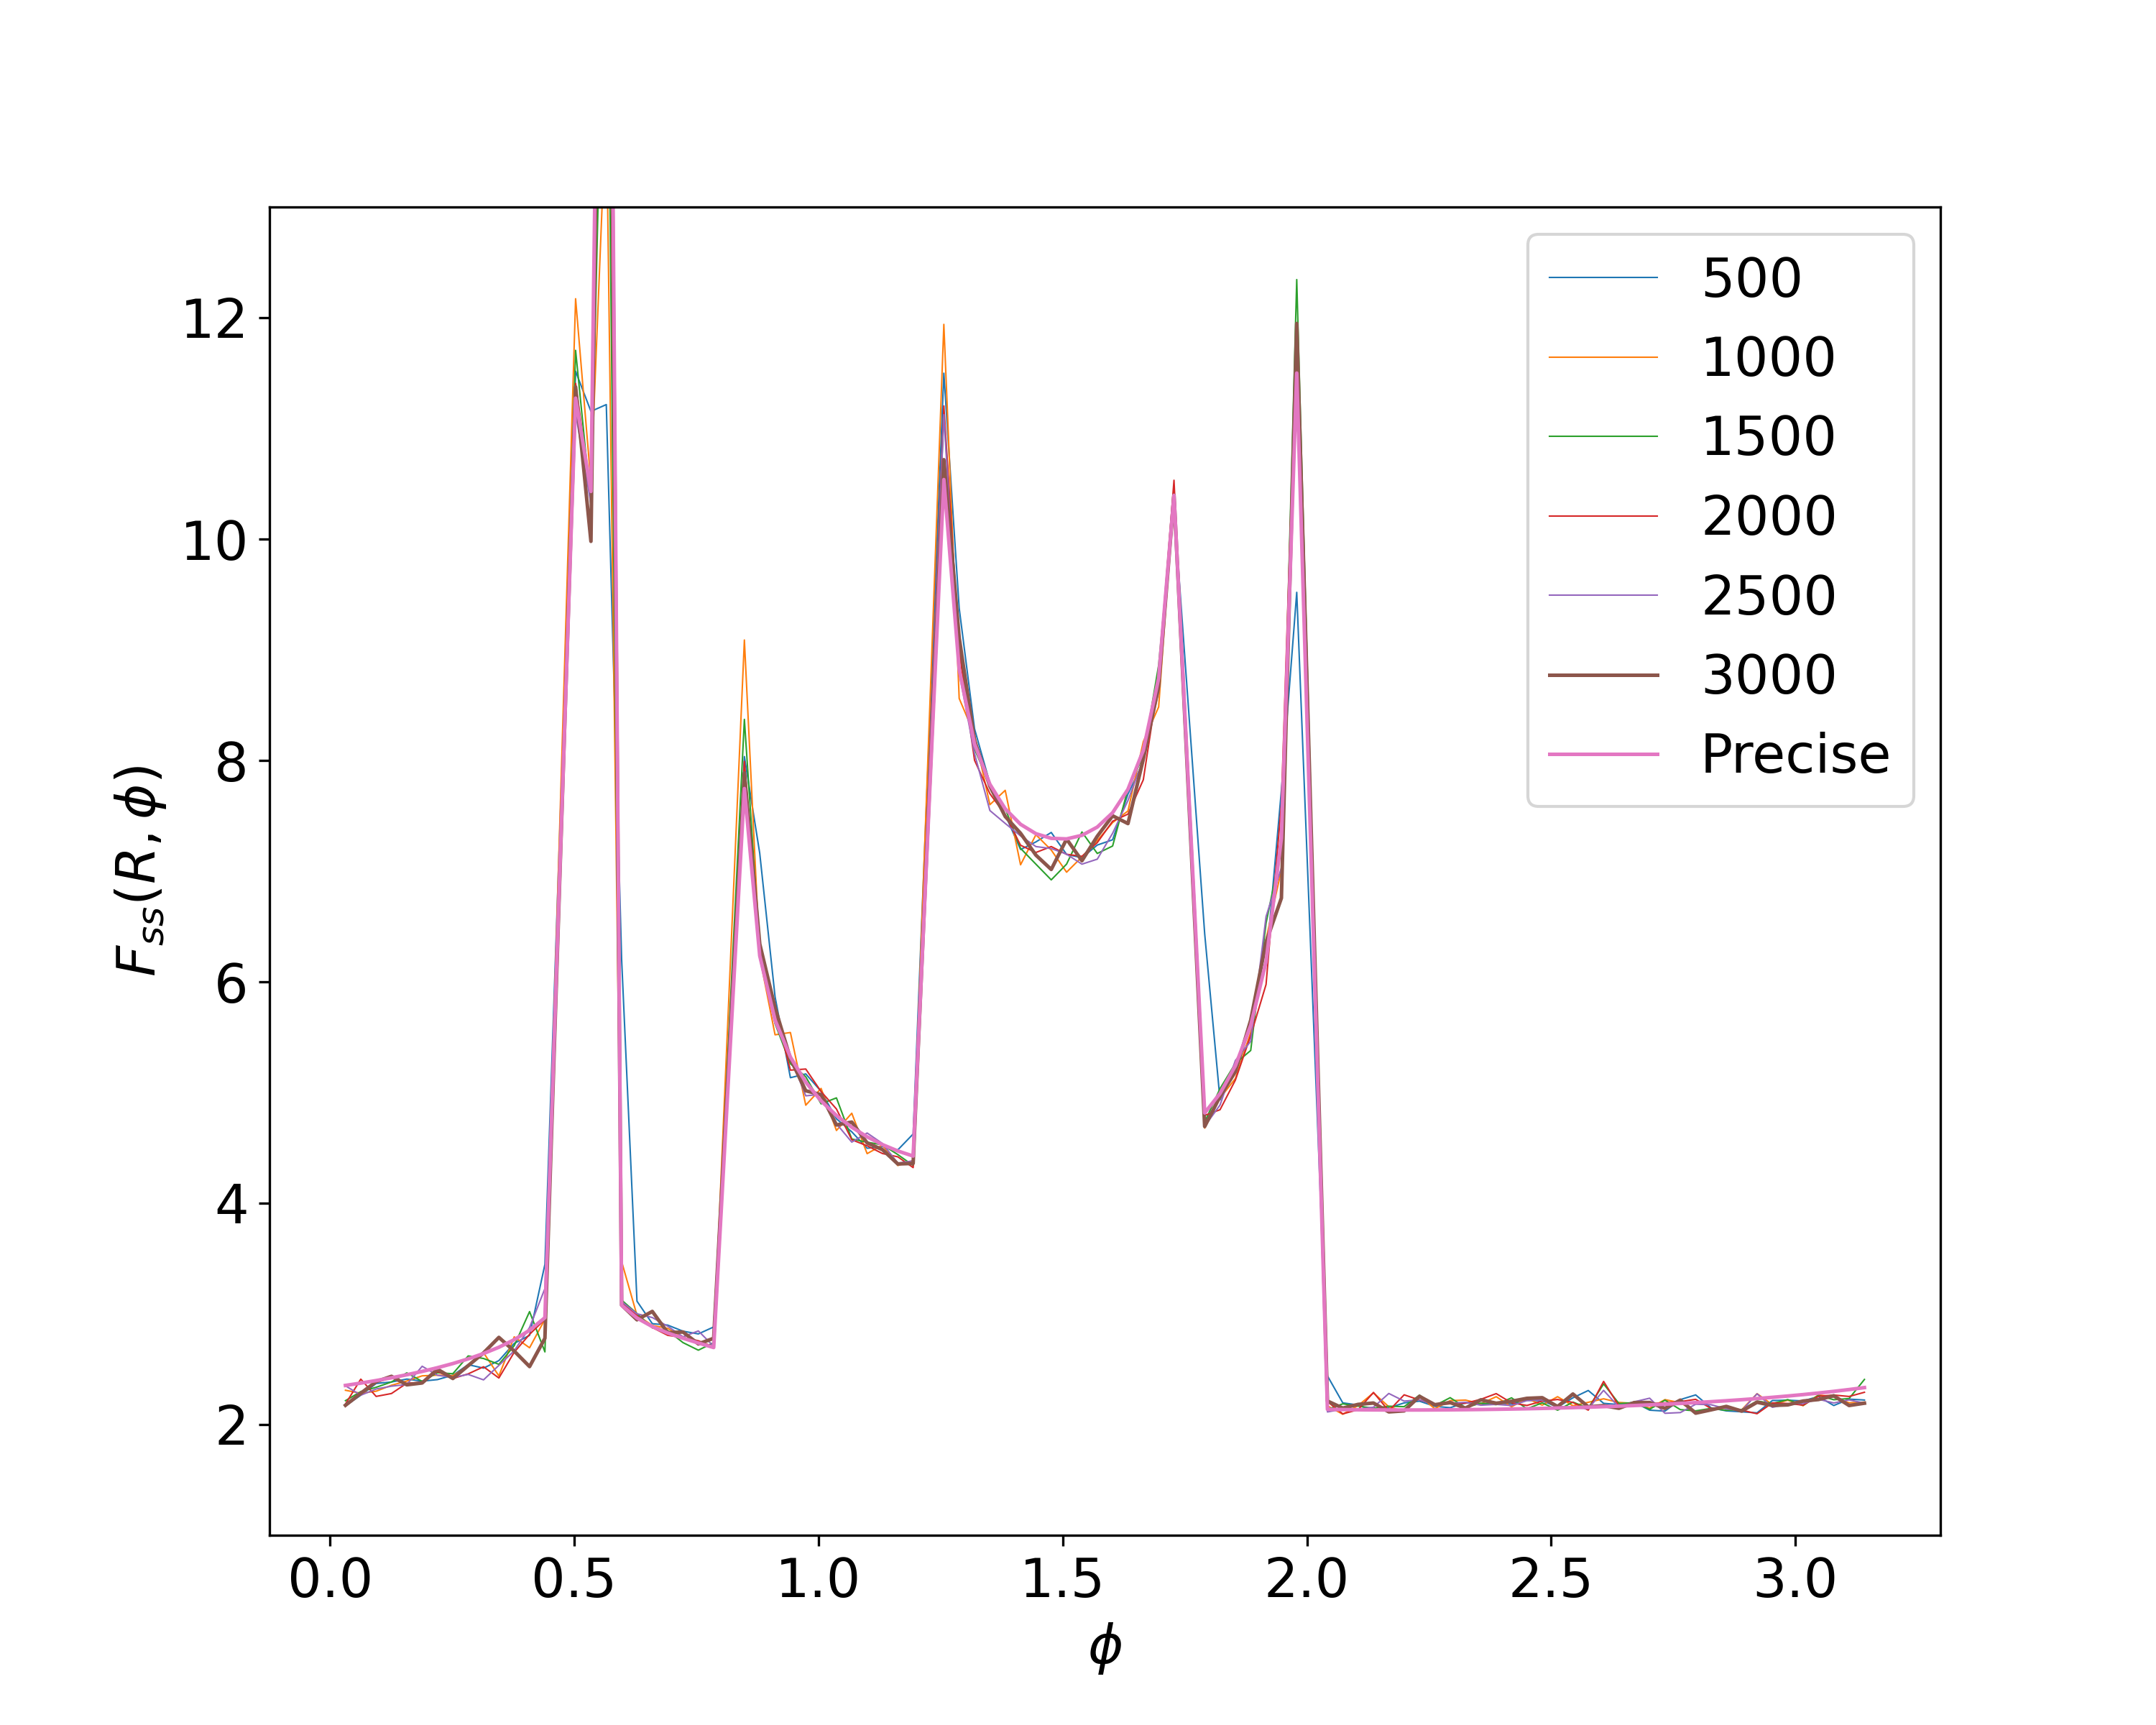
\includegraphics[width=0.45\linewidth]{images/fss-blob-5x5.png}
    \label{fig:fss-blob-5x5}}
  \caption[]{Plot of the surface-surface function for the blob on
    \cref{fig:blob}. Values of $F_{ss}$ were calculated in semi-circle with
    radius $R = 0.3$ and angle $\phi$ varying from $0$ to $\pi$. Resolution of
    the image varies from $500\times 500$ pixels to $3000\times 3000$.}
  \label{fig:fss-blob}
\end{figure*}

\subsection{Ellipses}
\label{sec:ellipses}
\begin{figure}
  \centering
  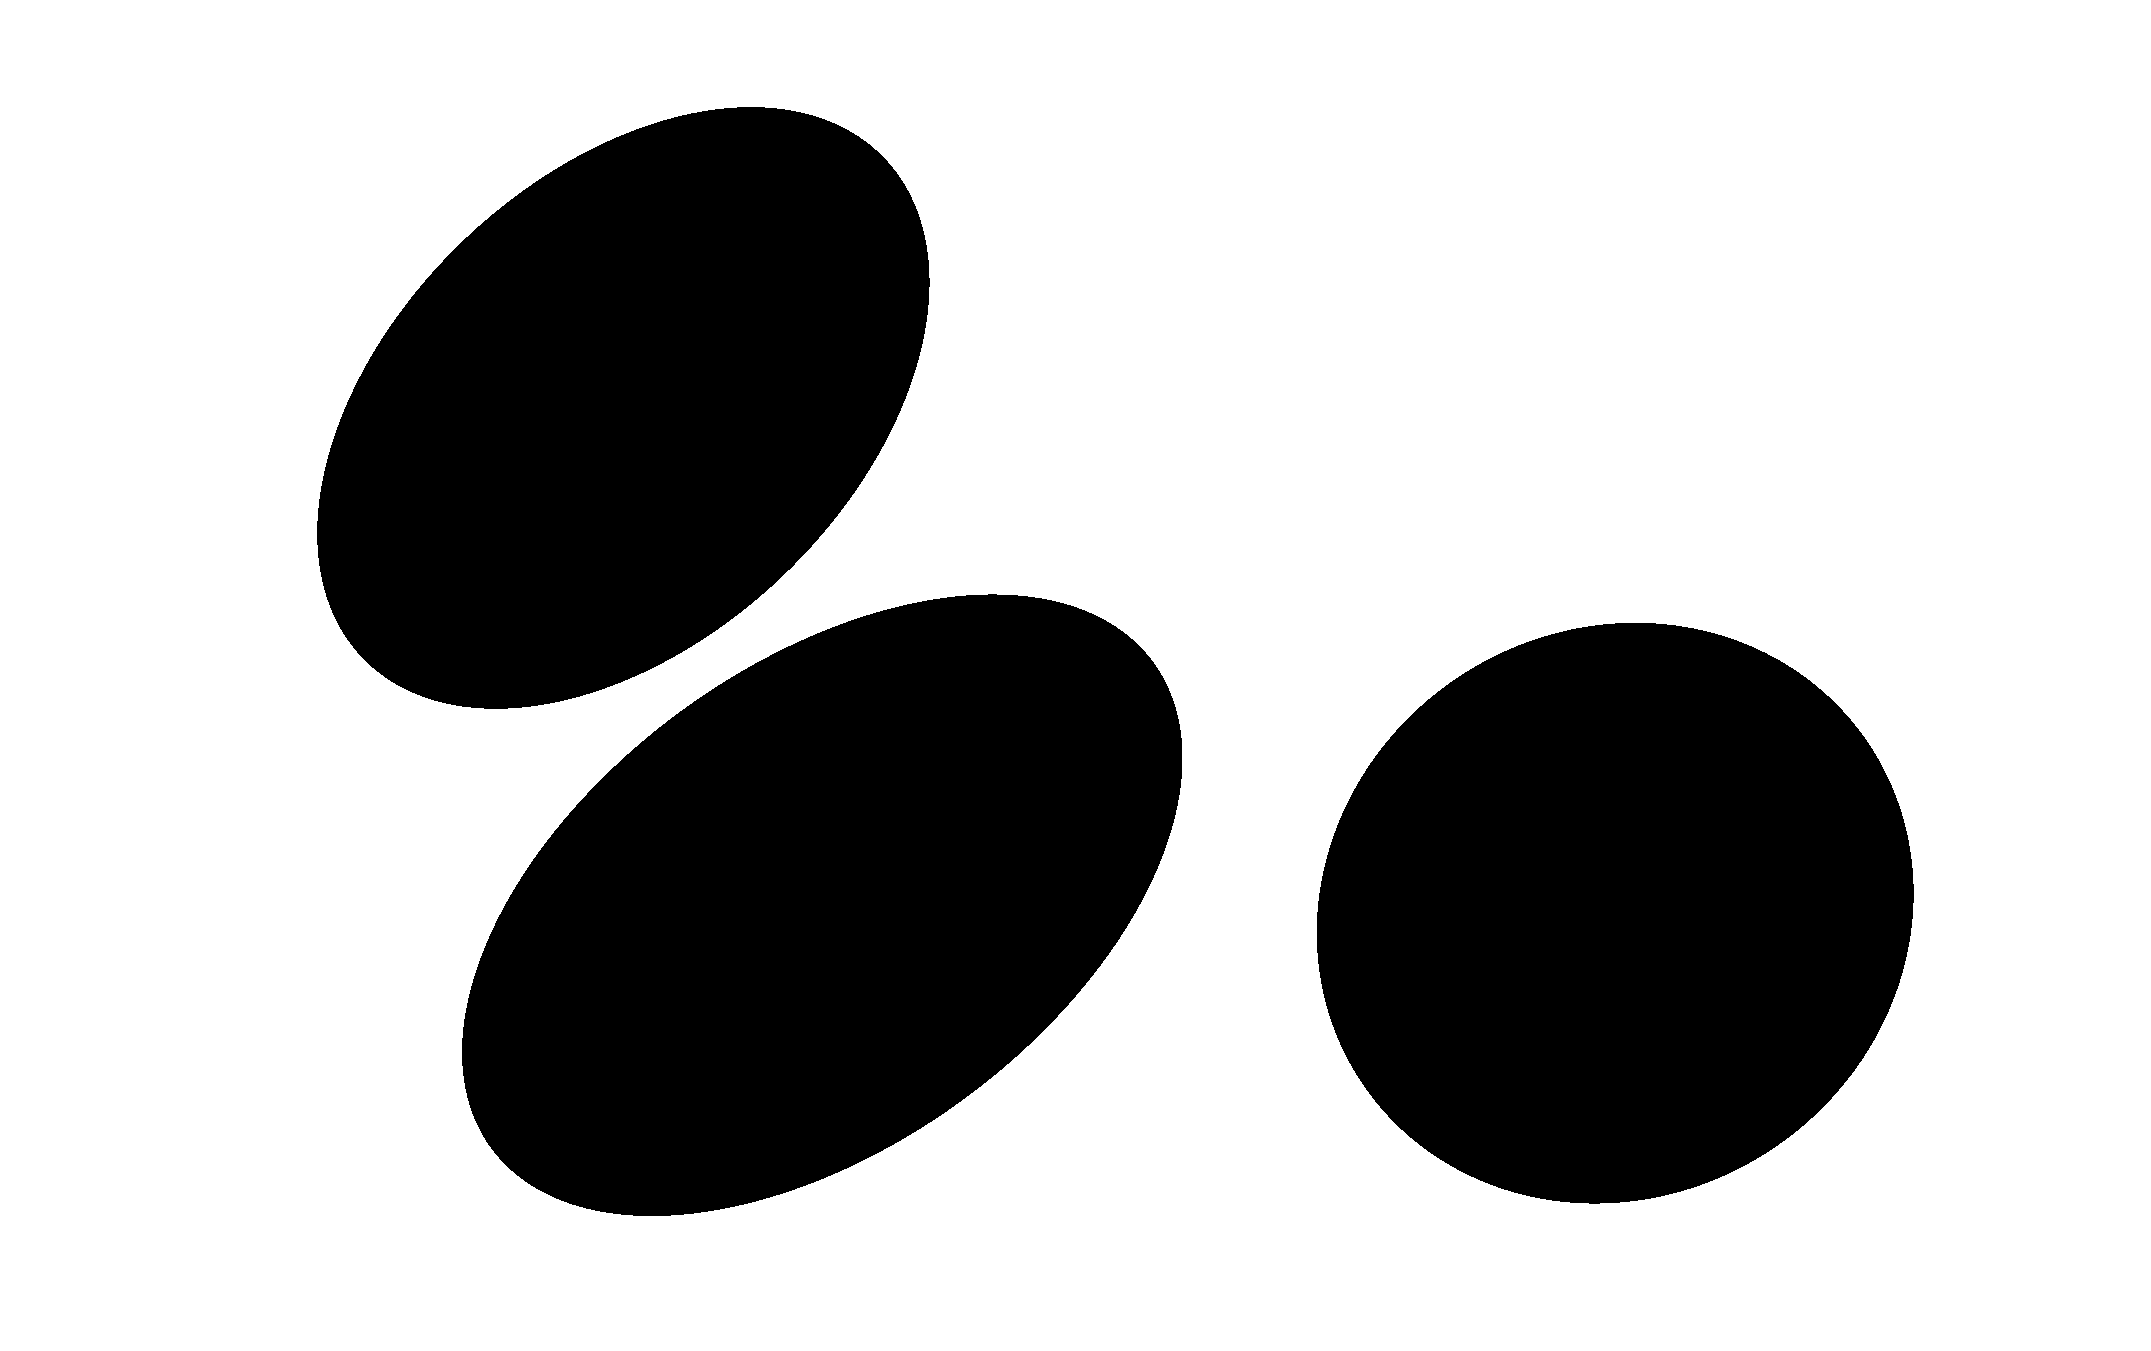
\includegraphics[width=0.8\linewidth, frame]{images/ellipses.png}
  \caption[]{An example of generated ellipses.}
  \label{fig:ellipses}
\end{figure}
Take $N$ random values $a_i$, $b_i$, $c_i$, $x^c_i$ and $y^c_i$ and define
\begin{equation*}
  f_i(x, y) = a_i(x-x^c_i)^2 + b(x-x^c_i)(y-y^c_i) + c_i(y-y^c_i)^2
\end{equation*}
with $a_ic_i - b_i^2 > 0$. Inequation
\begin{equation*}
  \min_i f_i(x, y) < A^2
\end{equation*}
defines $N$ ellipses like those which can be seen on \cref{fig:ellipses}. A
comparison between two algorithms is on \cref{fig:fss-ellipses}.
\begin{figure*}[!pt]
  \centering
  \subfigure[$3\times 3$ kernel $H$]{
    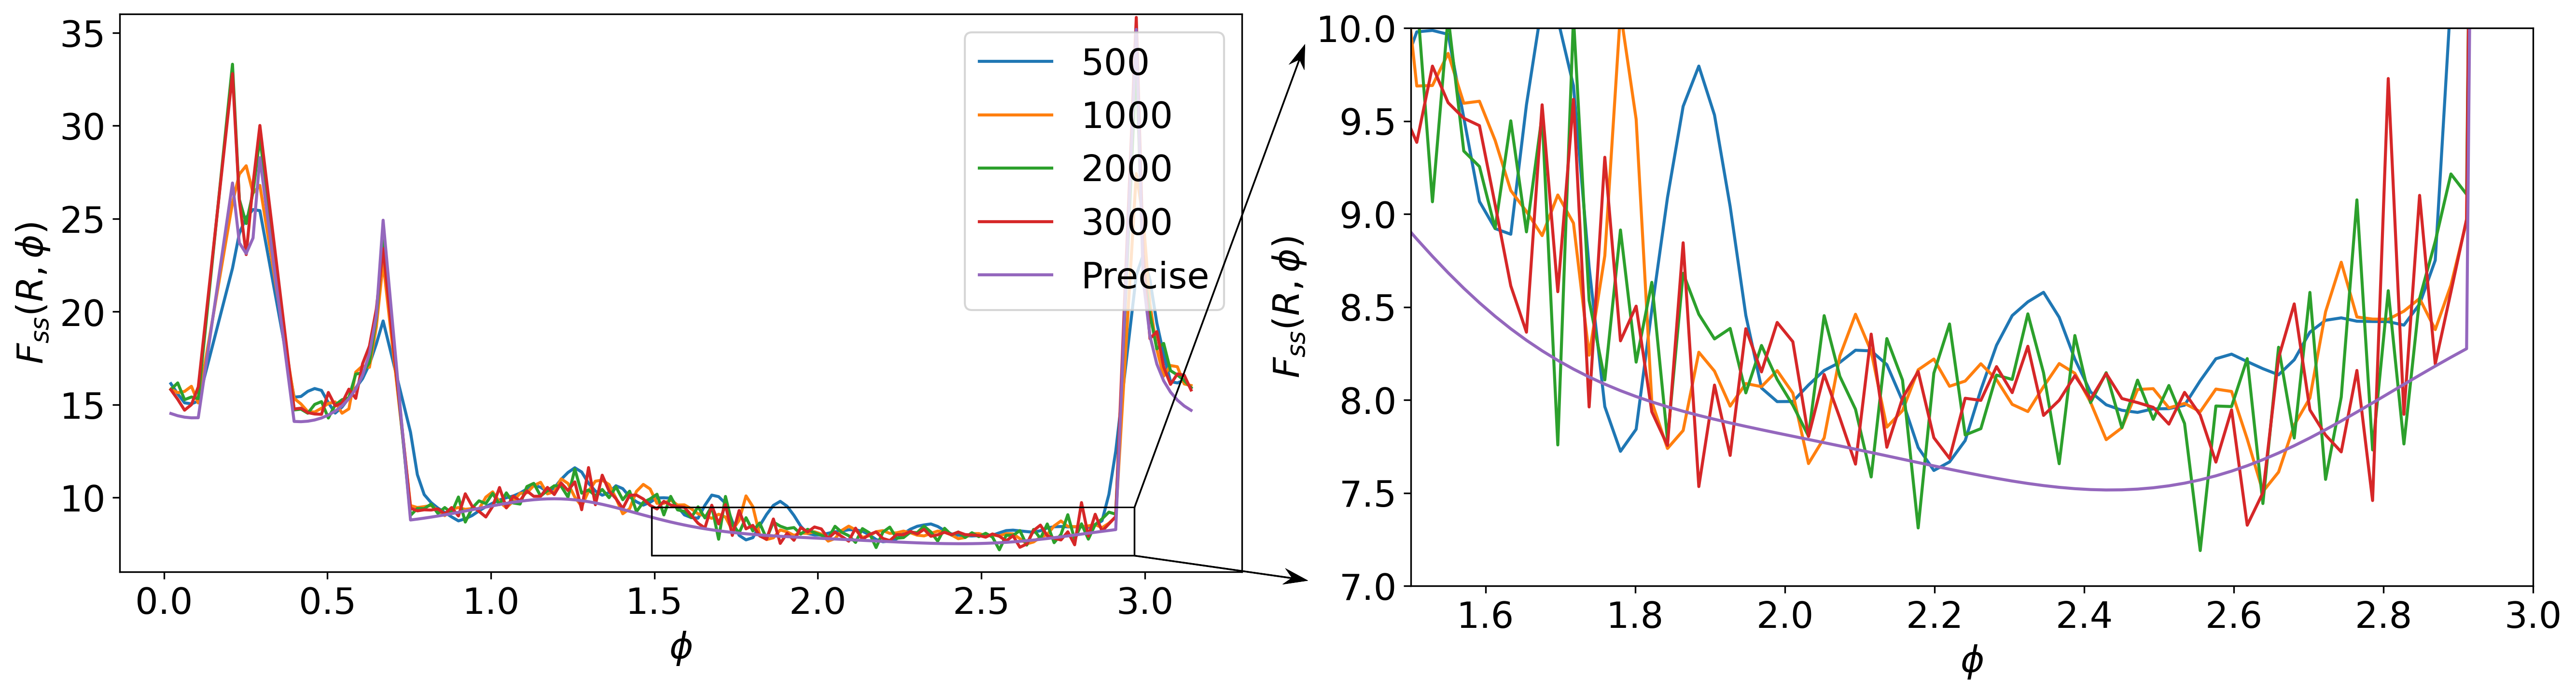
\includegraphics[width=0.45\linewidth]{images/fss-ellipses-3x3.png}
    \label{fig:fss-ellipses-3x3}}
  \hfill
  \subfigure[$5\times 5$ kernel $H'$]{
    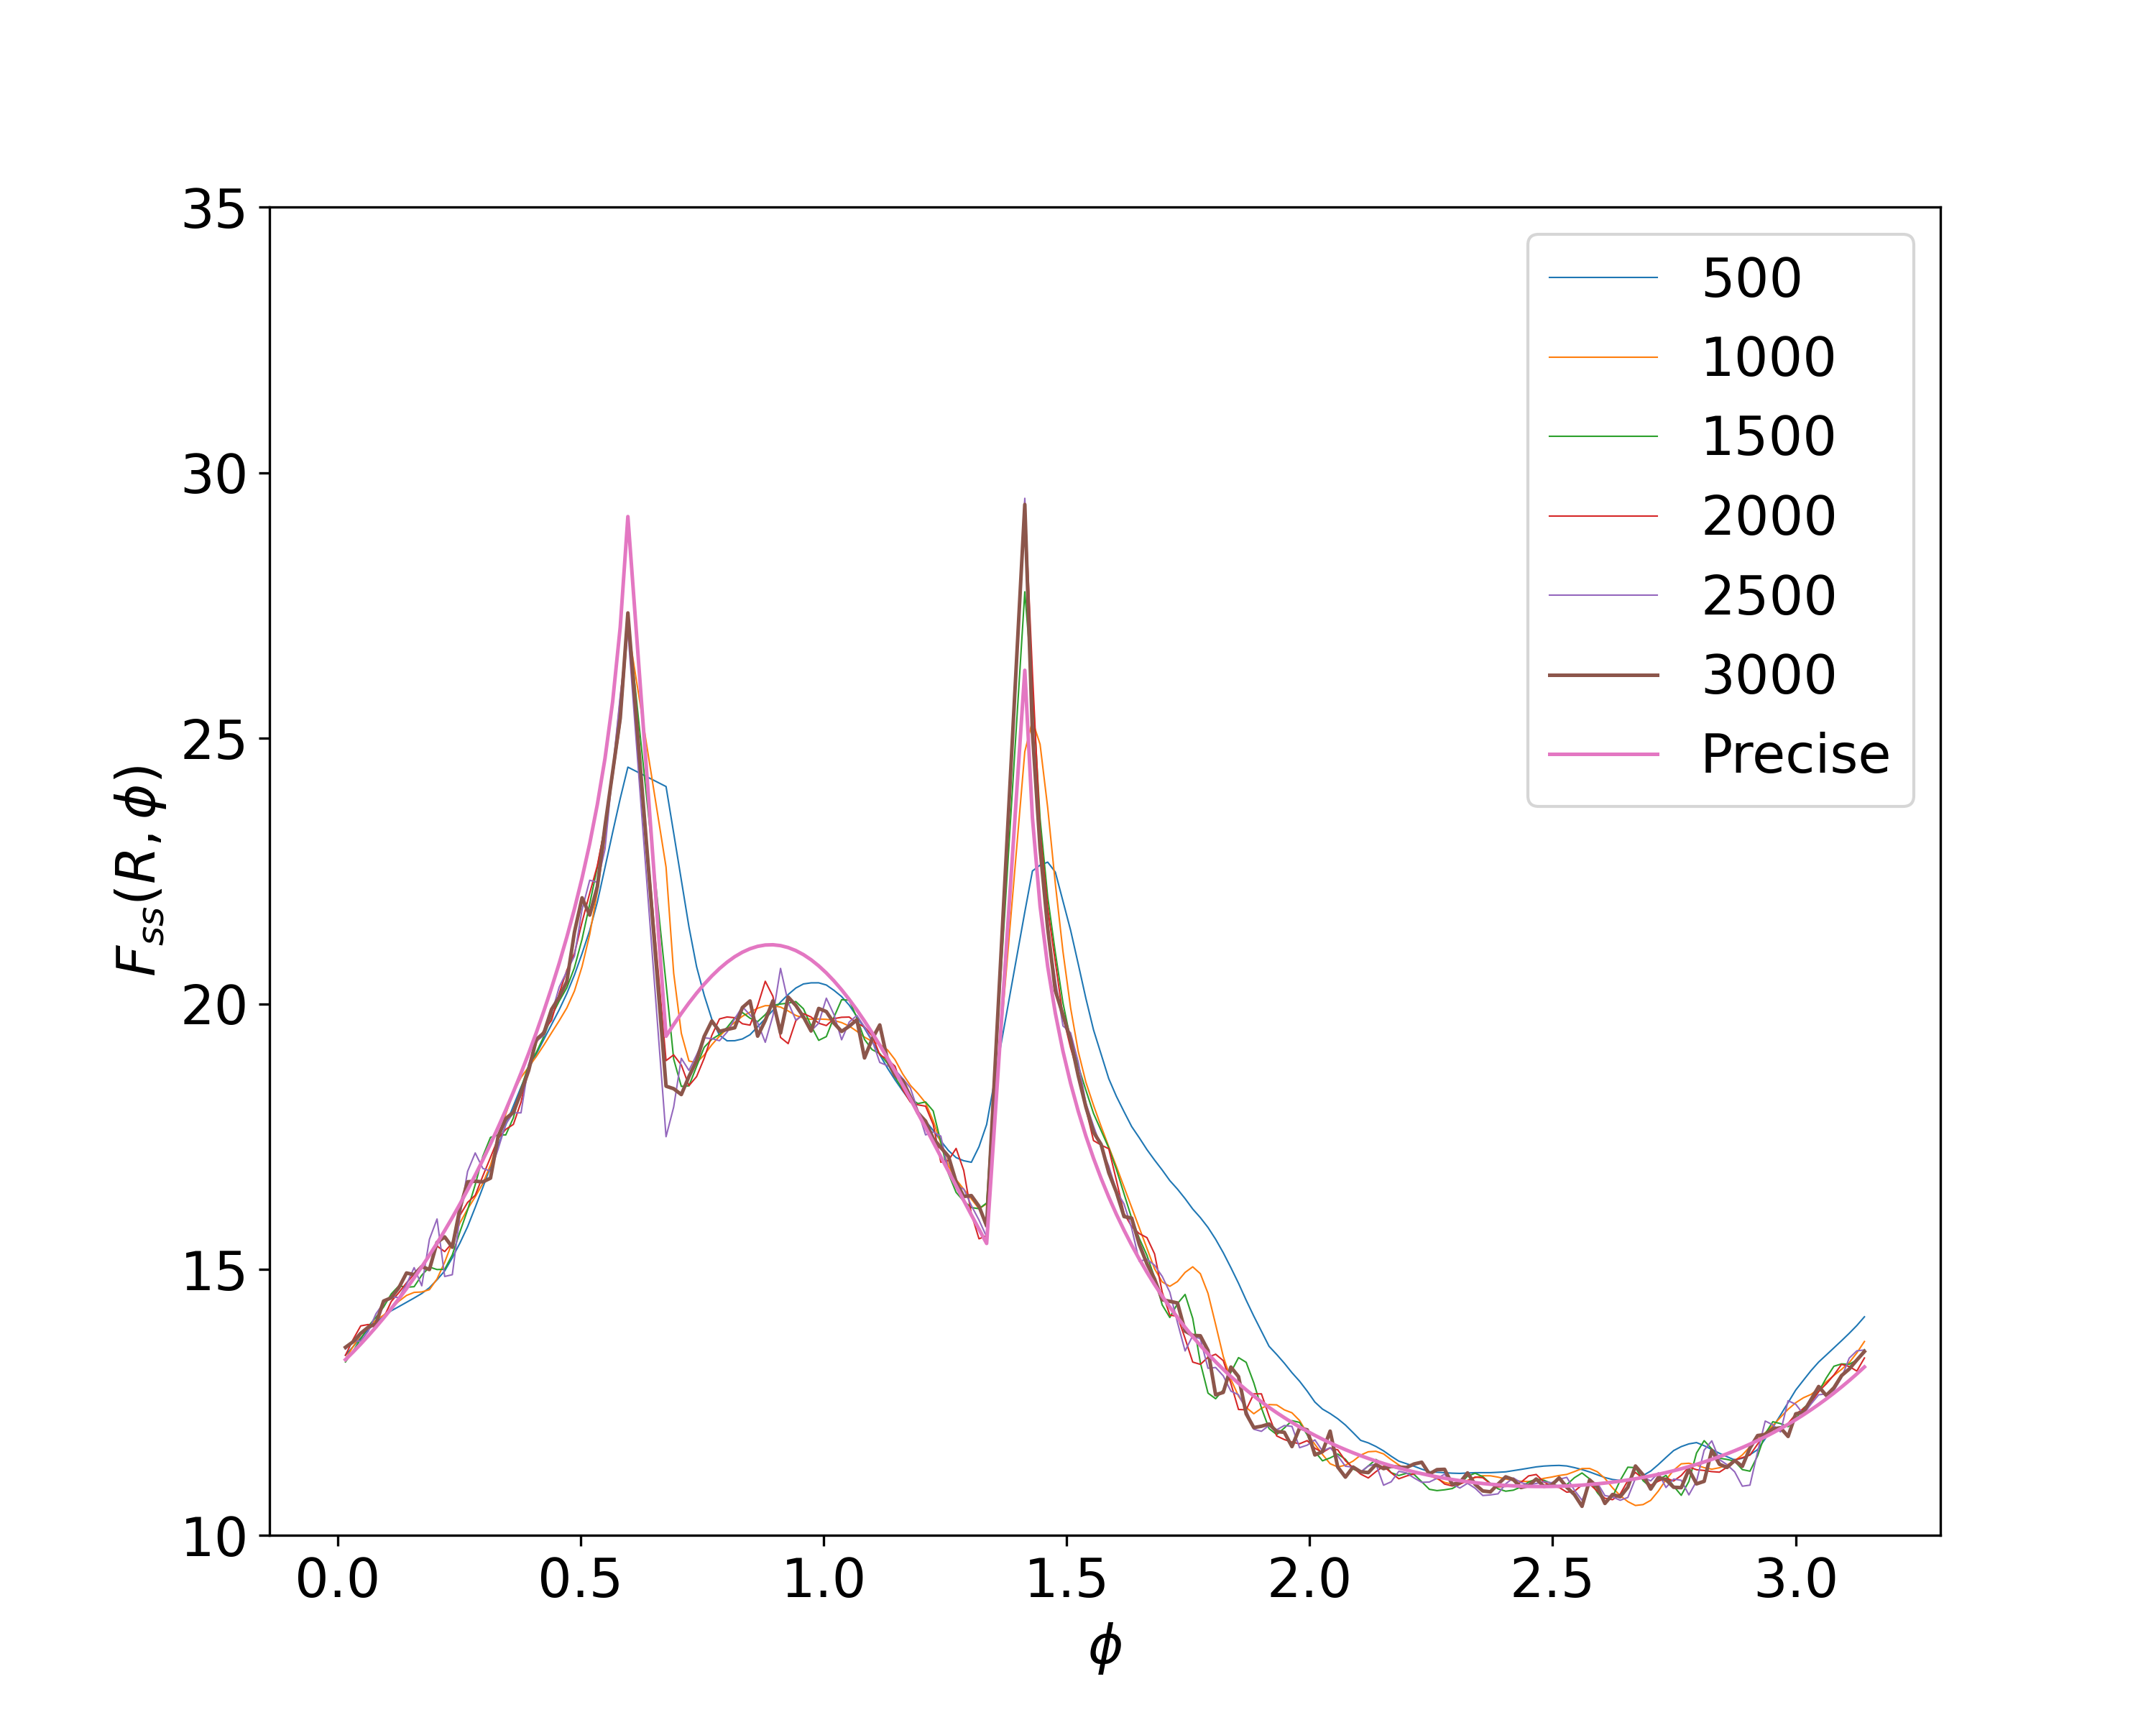
\includegraphics[width=0.45\linewidth]{images/fss-ellipses-5x5.png}
    \label{fig:fss-ellipses-5x5}}
  \caption[]{Plot of the surface-surface function for ellipses on
    \cref{fig:ellipses}. Values of $F_{ss}$ were calculated in semi-circle with
    radius $R = 0.1$ and angle $\phi$ varying from $0$ to $\pi$. Resolution of
    the image varies from $500\times 500$ pixels to $3000\times 3000$.}
  \label{fig:fss-ellipses}
\end{figure*}

\section{Improvement of the fast algorithm}
\label{sec:improvement}
\begin{figure}
  \centering
  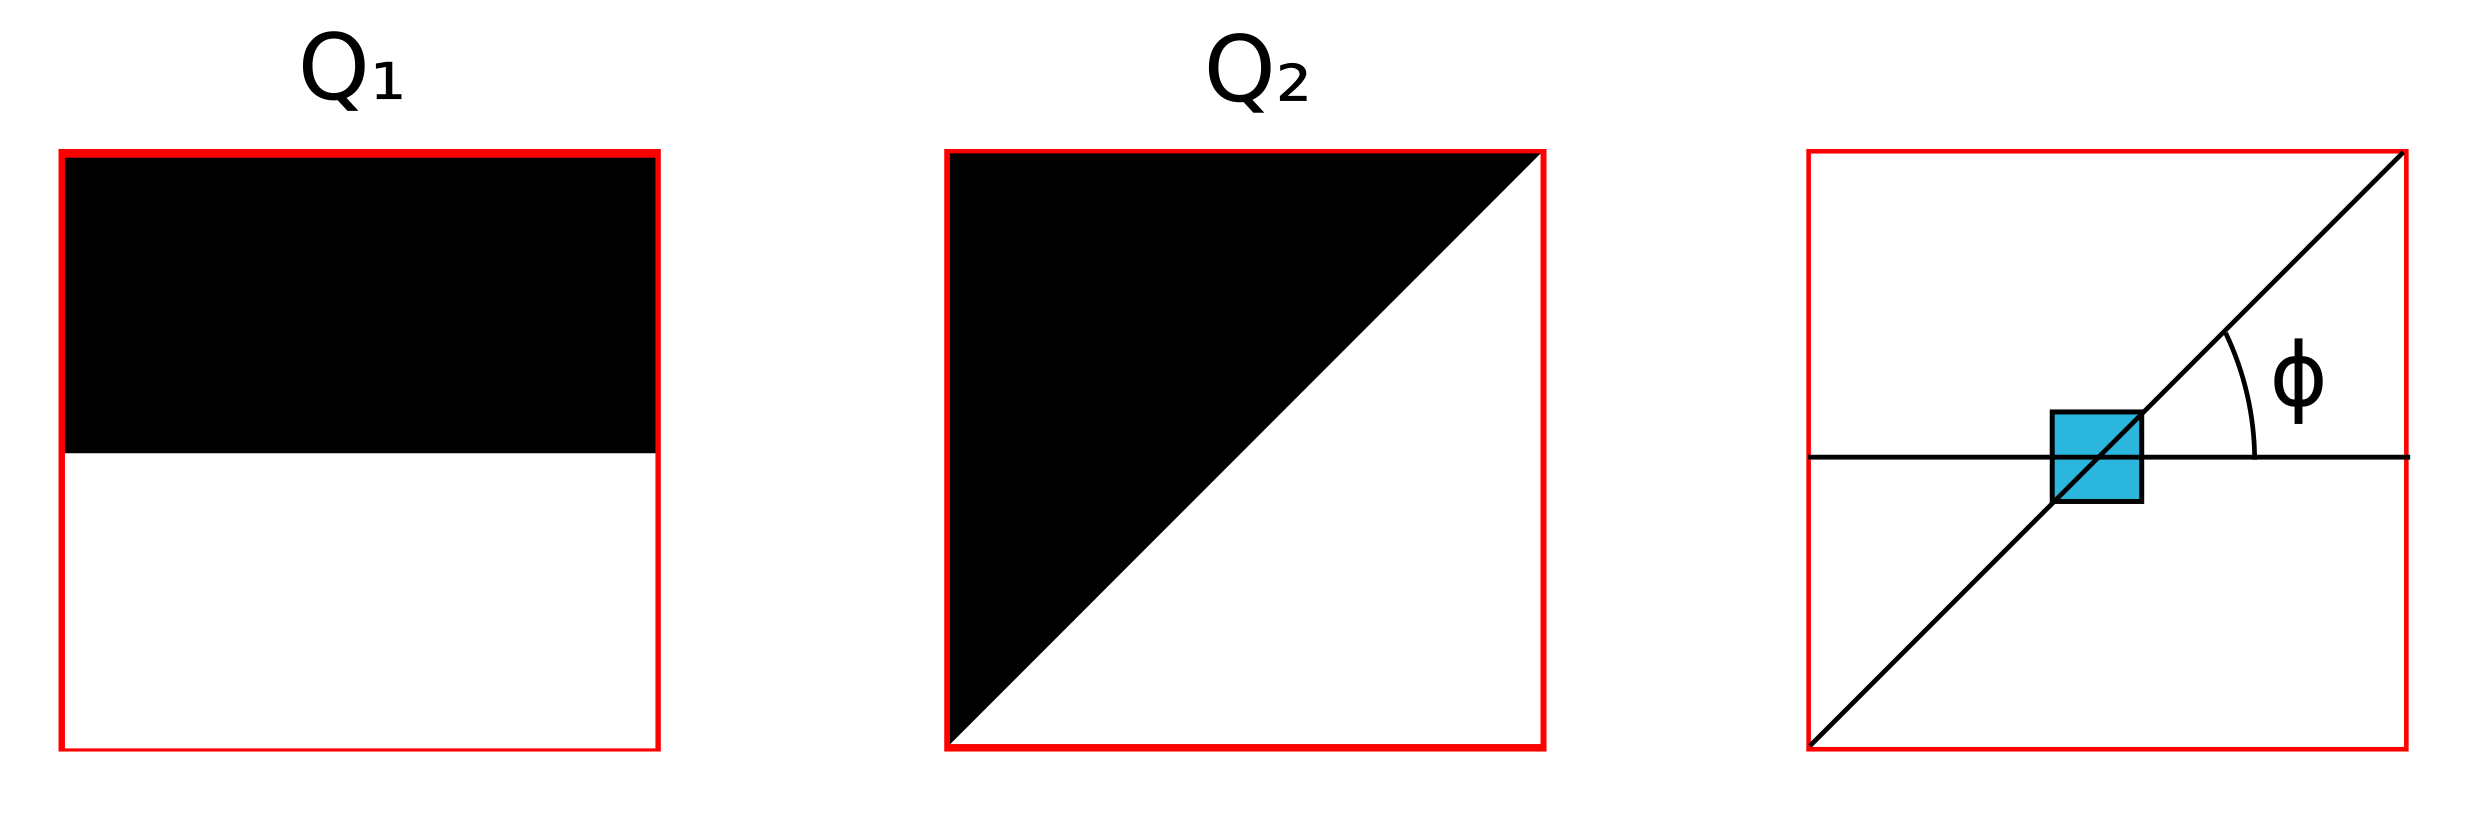
\includegraphics[width=0.8\linewidth]{images/experiment-setup.png}
  \caption[]{Left, center: images $A$ and $B$ used in the experiment described
    in \cref{sec:improvement}. Right: Interfaces between phases are line
    segments which intersect each other at angle $\phi$. Shaded area is where
    $(H*A)\cdot(H*B)$ has non-zero values.}
  \label{fig:experiment-setup}
\end{figure}
Take two 2D images like the ones on \cref{fig:experiment-setup}. Boundaries
between black and white cross each other at the angle $\phi$. We apply the
filter $H$ (\cref{eq:filter-3x3-2d}) to each image, multiply results
element-wise and sum all elements of the product. An obtained value must
approximate $1/\sin \phi$ if we want $H$ to be suitable for calculation of
surface-surface function. With filter described in \cref{sec:algo} we get a
picture as on \cref{fig:angles-3x3}. We see that $H$ approximates
$1/\sin \phi$ not very good.

Now, let's try a wider filter $H'$:
\begin{align}
  H'_{ij} &= \frac{1}{30} \left[
    \begin{array}{ccccc}
      1 & 1 & 1 & 1 & 1 \\
      1 & 1 & 1 & 1 & 1 \\
      1 & 1 & -24 & 1 & 1 \\
      1 & 1 & 1 & 1 & 1 \\
      1 & 1 & 1 & 1 & 1 \\
    \end{array}
    \right] \label{eq:filter-5x5-2d} \\
  H'_{ijk} &= \frac{1}{150} \left[
    \begin{array}{ccccc}
      1 & 1 & 1 & 1 & 1 \\
      1 & 1 & 1 & 1 & 1 \\
      1 & 1 & 1 & 1 & 1 \\
      1 & 1 & 1 & 1 & 1 \\
      1 & 1 & 1 & 1 & 1 \\
    \end{array} ;
    \begin{array}{ccccc}
      1 & 1 & 1 & 1 & 1 \\
      1 & 1 & 1 & 1 & 1 \\
      1 & 1 & -124 & 1 & 1 \\
      1 & 1 & 1 & 1 & 1 \\
      1 & 1 & 1 & 1 & 1 \\
    \end{array} ;
    \begin{array}{ccccc}
      1 & 1 & 1 & 1 & 1 \\
      1 & 1 & 1 & 1 & 1 \\
      1 & 1 & 1 & 1 & 1 \\
      1 & 1 & 1 & 1 & 1 \\
      1 & 1 & 1 & 1 & 1 \\
    \end{array}
    \right] \label{eq:filter-5x5-3d}
\end{align}
With this filter we get a different picture (\cref{fig:angles-5x5}). A
comparison of the fast algorithm with a wider filter kernel with a precise
calculation for a ``blob'' described in \cref{sec:gauss} is show on
\cref{fig:fss-blob-5x5}. A case with ellipses from \cref{sec:ellipses} is on
\cref{fig:fss-ellipses-5x5}.
\begin{figure*}[!pt]
  \centering
  \subfigure[$3\times 3$ kernel $H$]{
    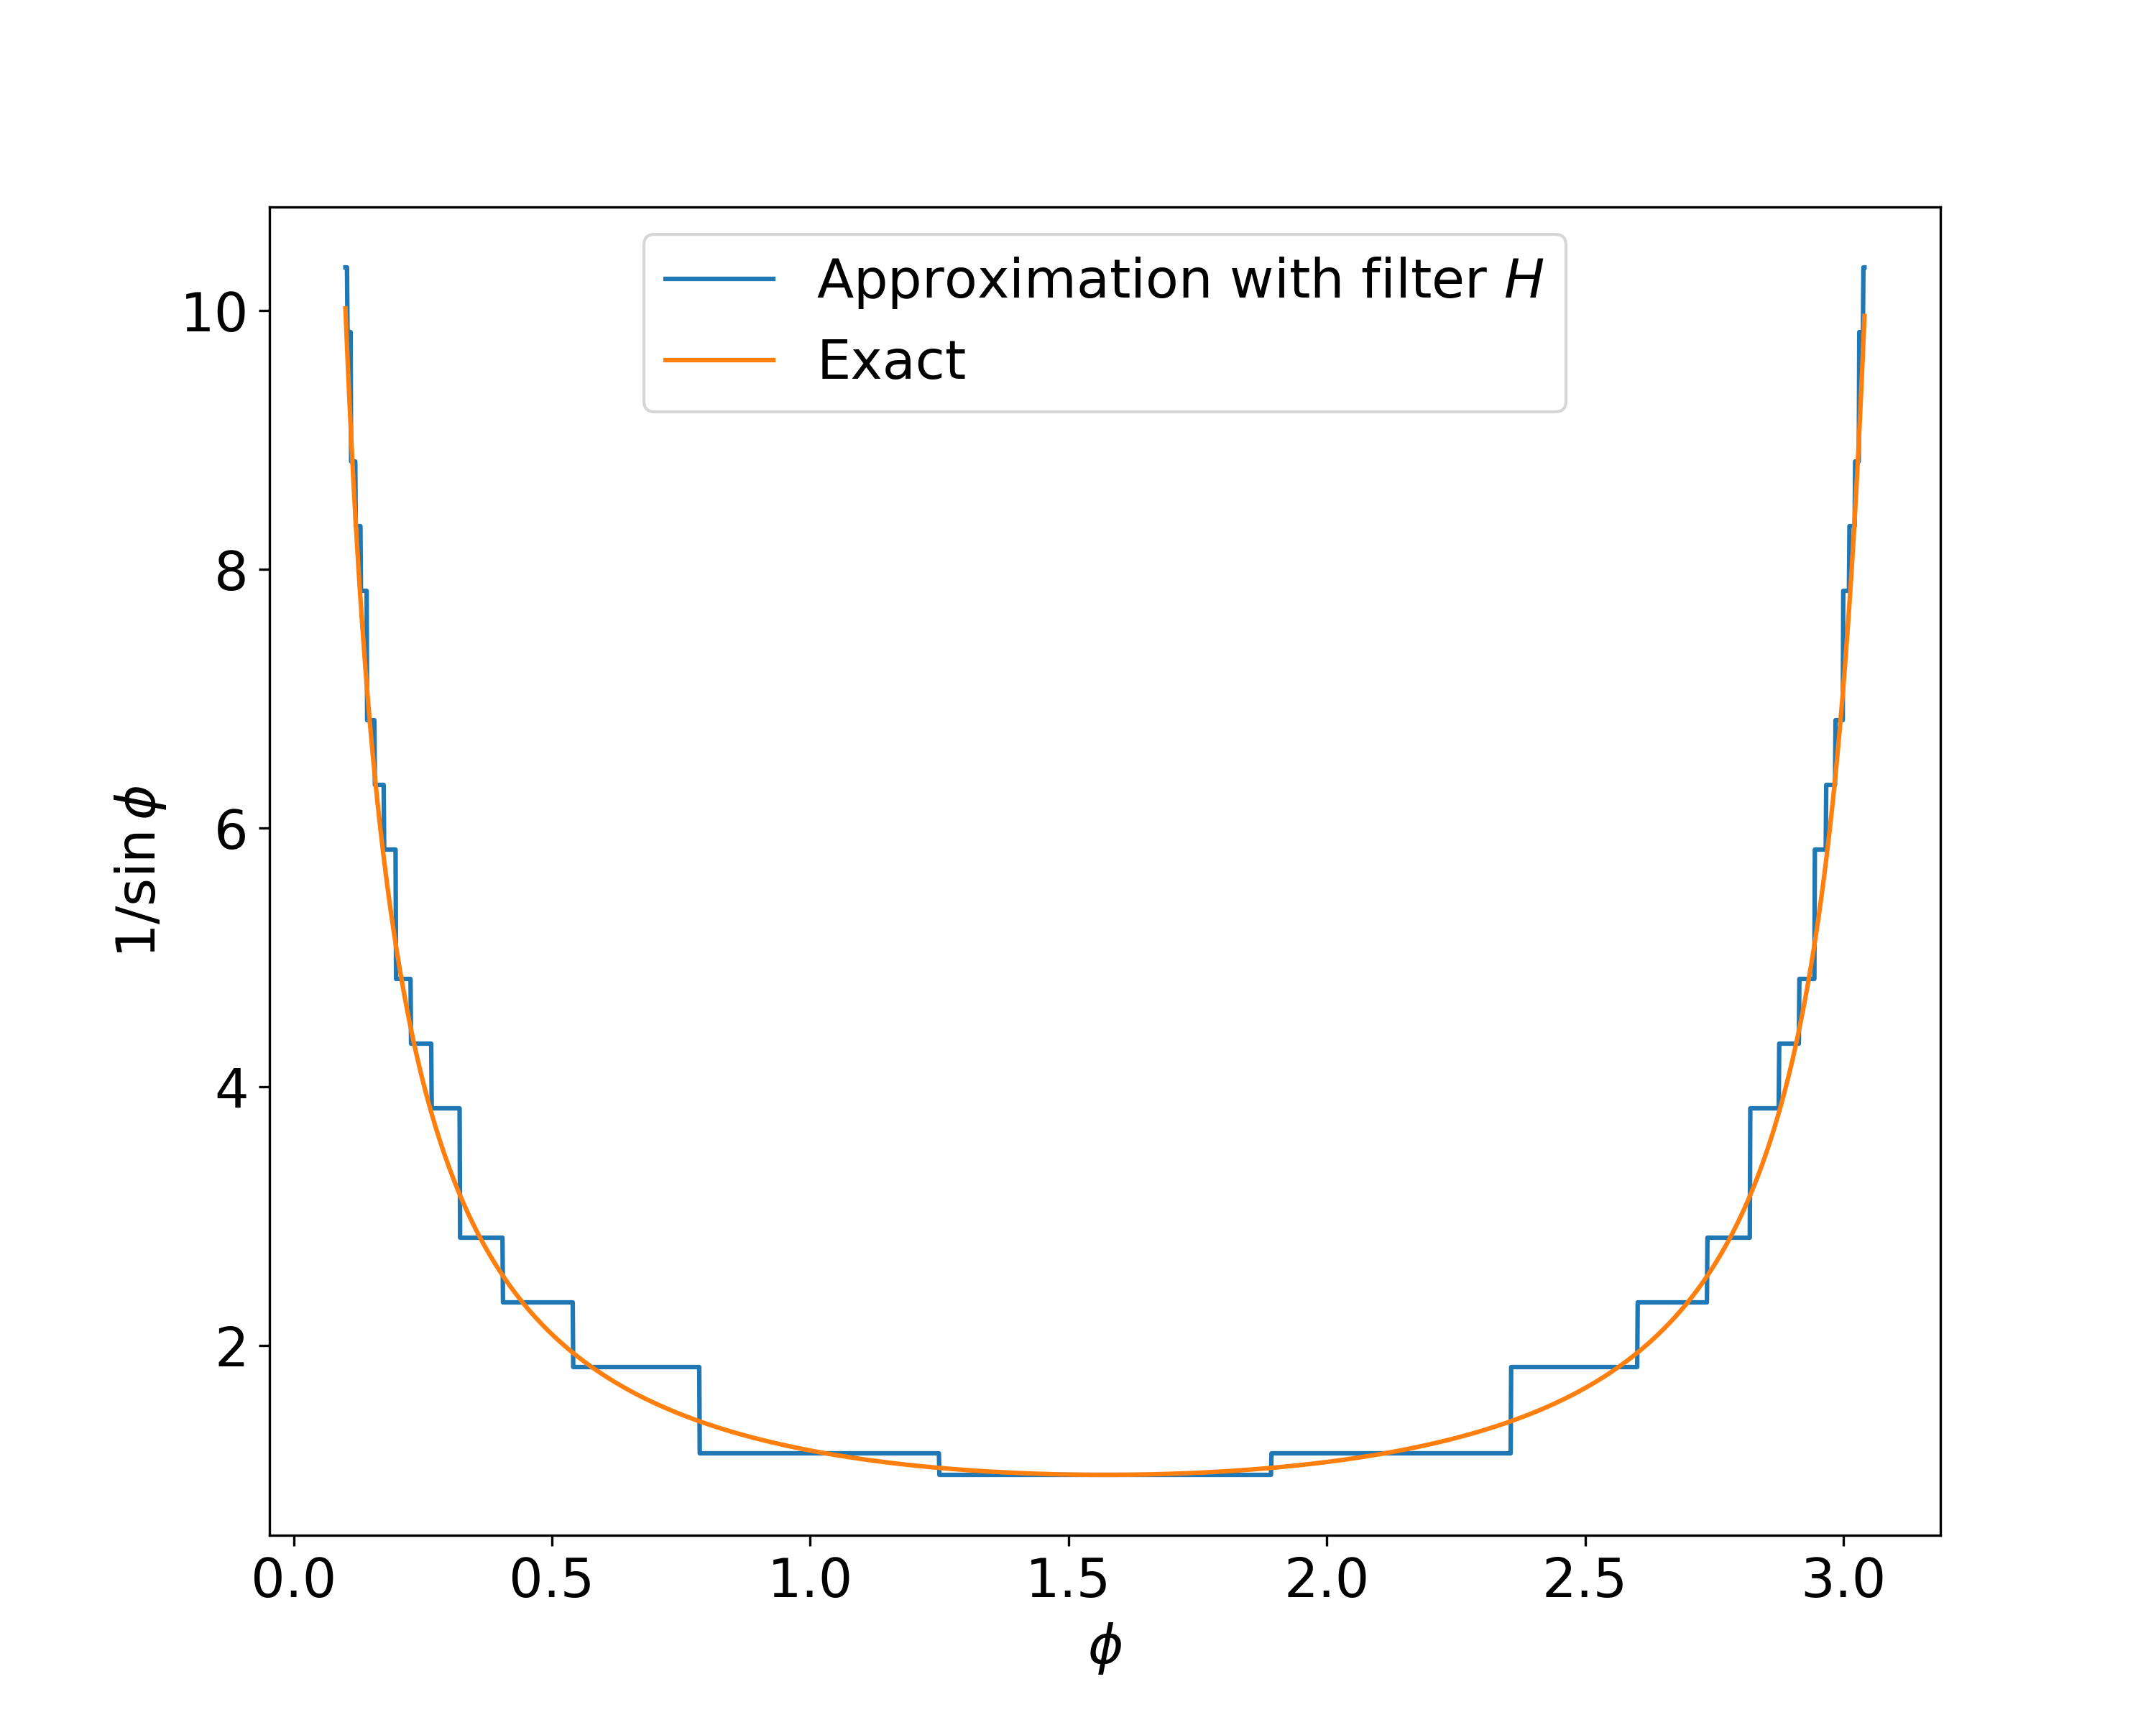
\includegraphics[width=0.45\linewidth]{images/angles-3x3.png}
    \label{fig:angles-3x3}}
  \hfill
  \subfigure[$5\times 5$ kernel $H'$]{
    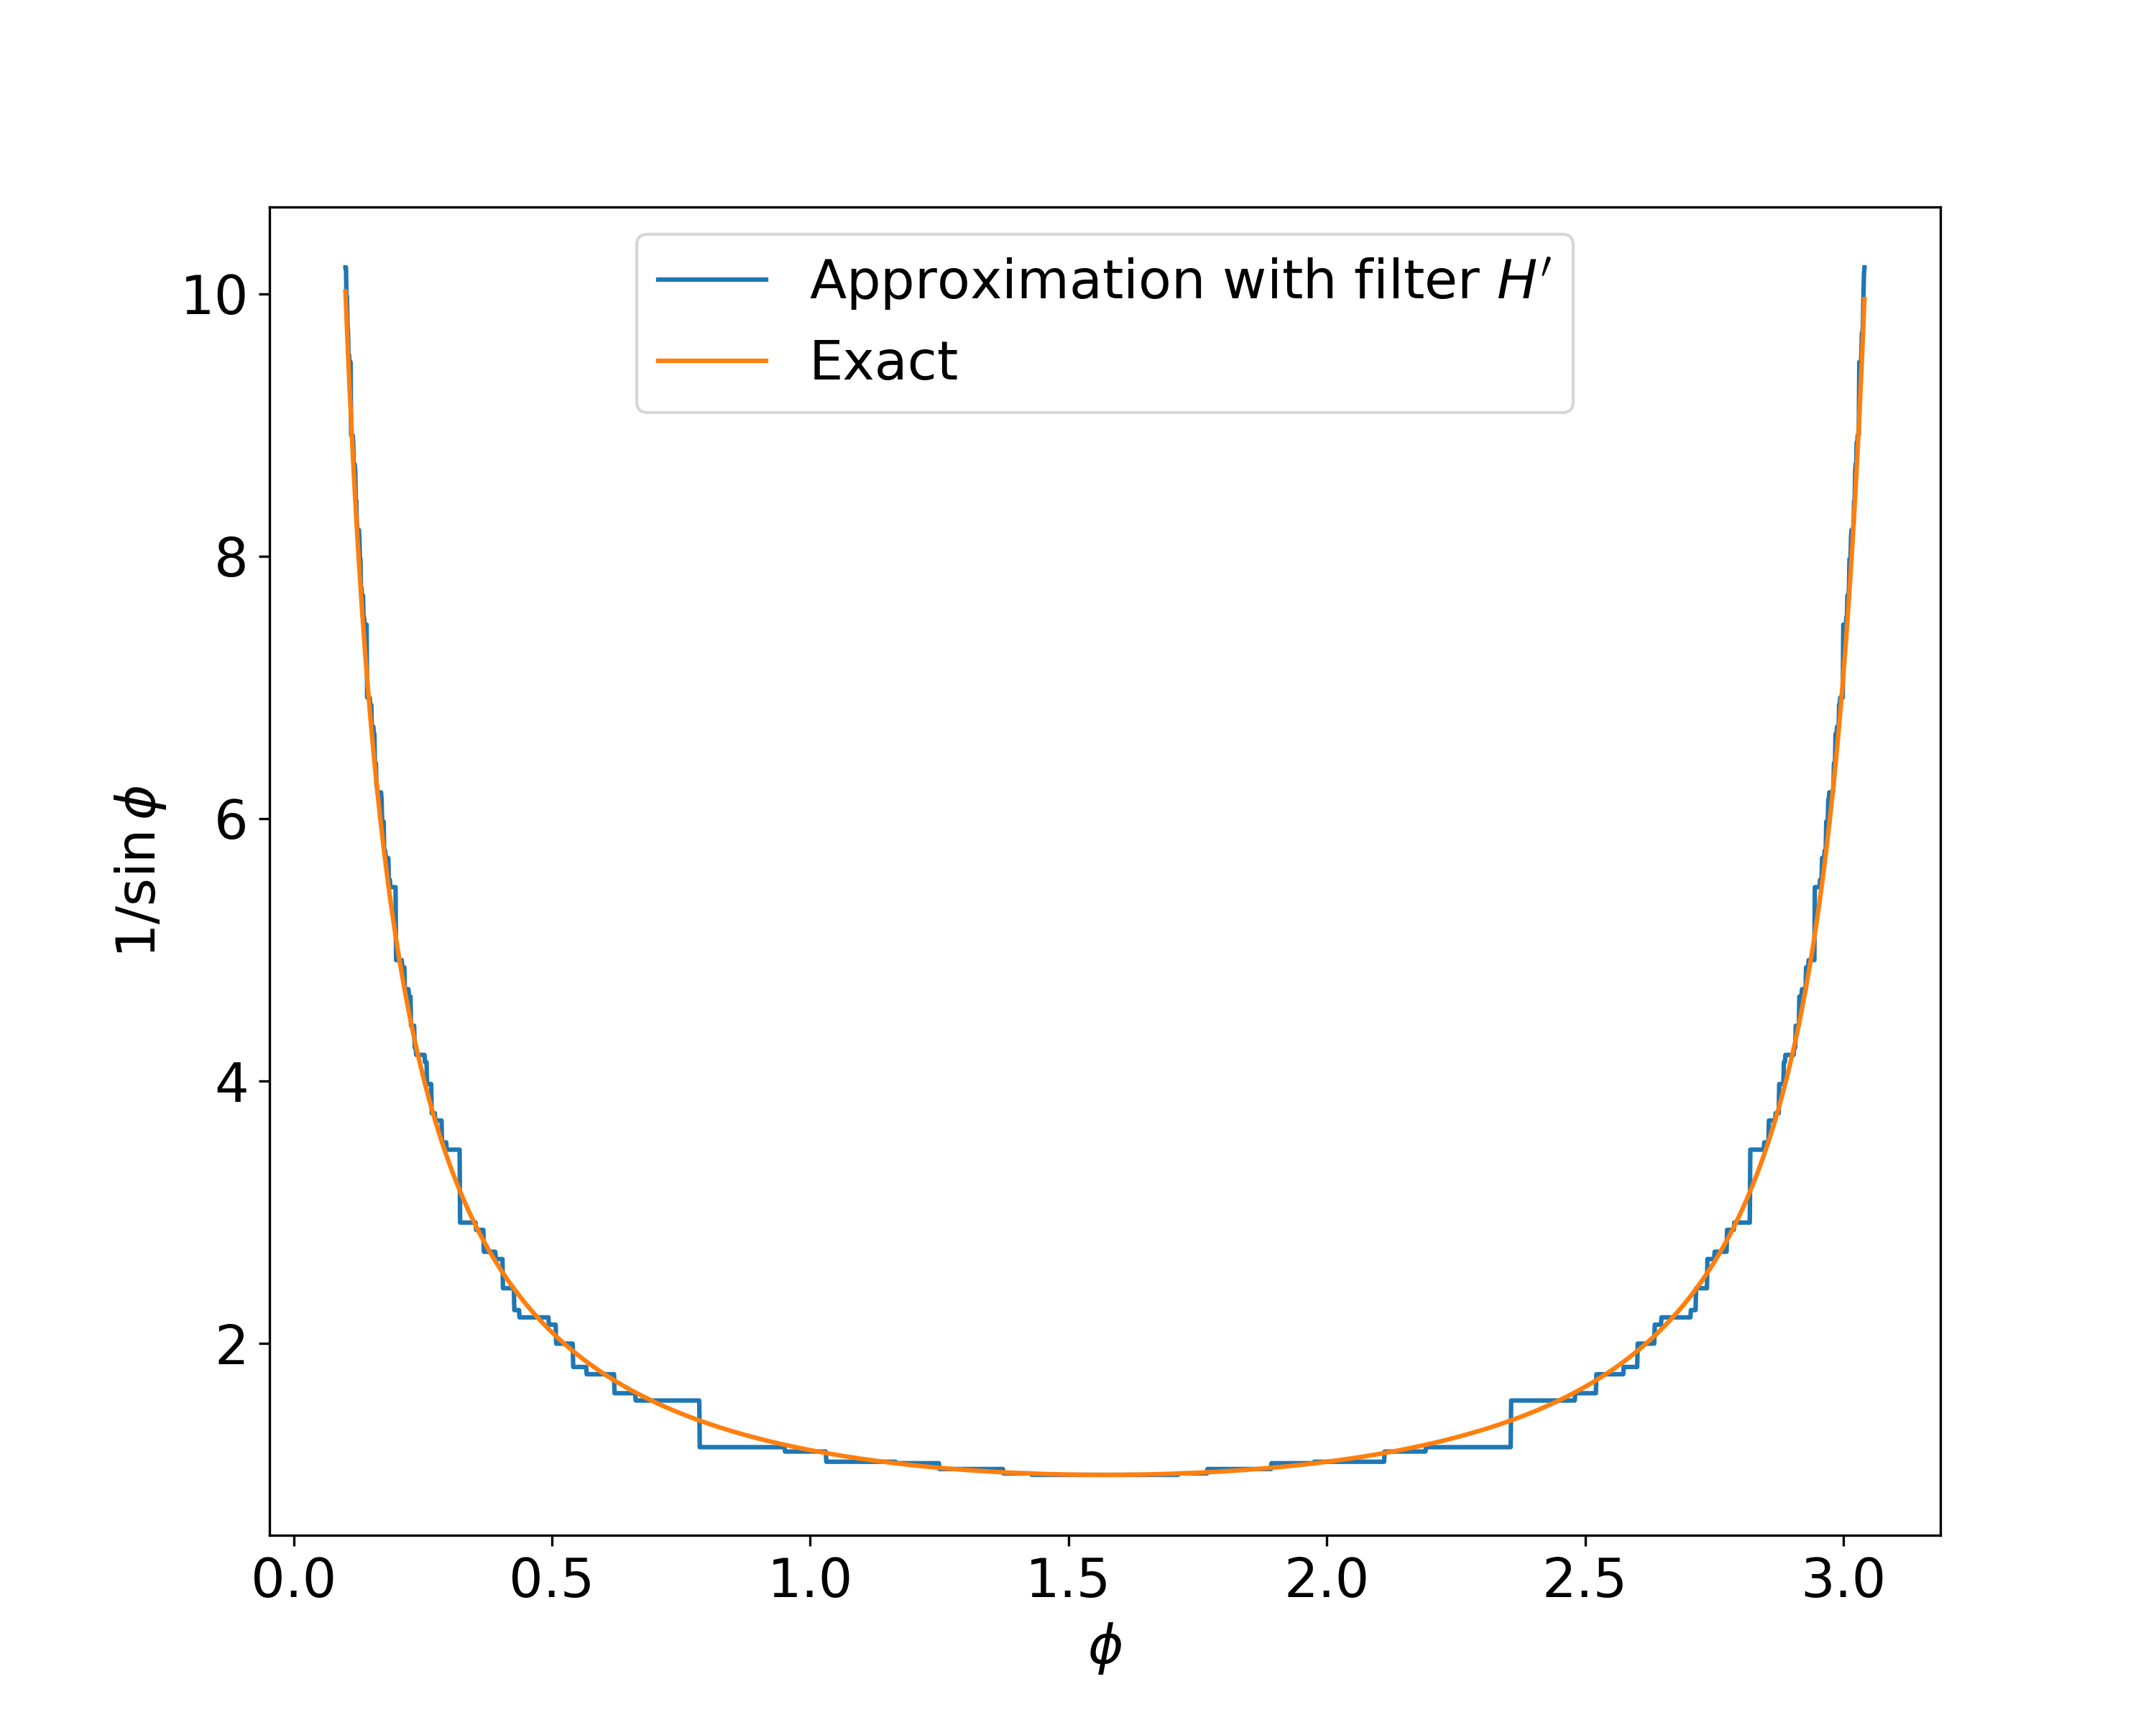
\includegraphics[width=0.45\linewidth]{images/angles-5x5.png}
    \label{fig:angles-5x5}}
  \caption[]{Estimation of $1/\sin\phi$ where $\phi$ is the angle between
    tangent lines to the interface by filters $H$ and $H'$.}
  \label{fig:angles}
\end{figure*}

\section{Results}
\begin{figure}
  \centering
  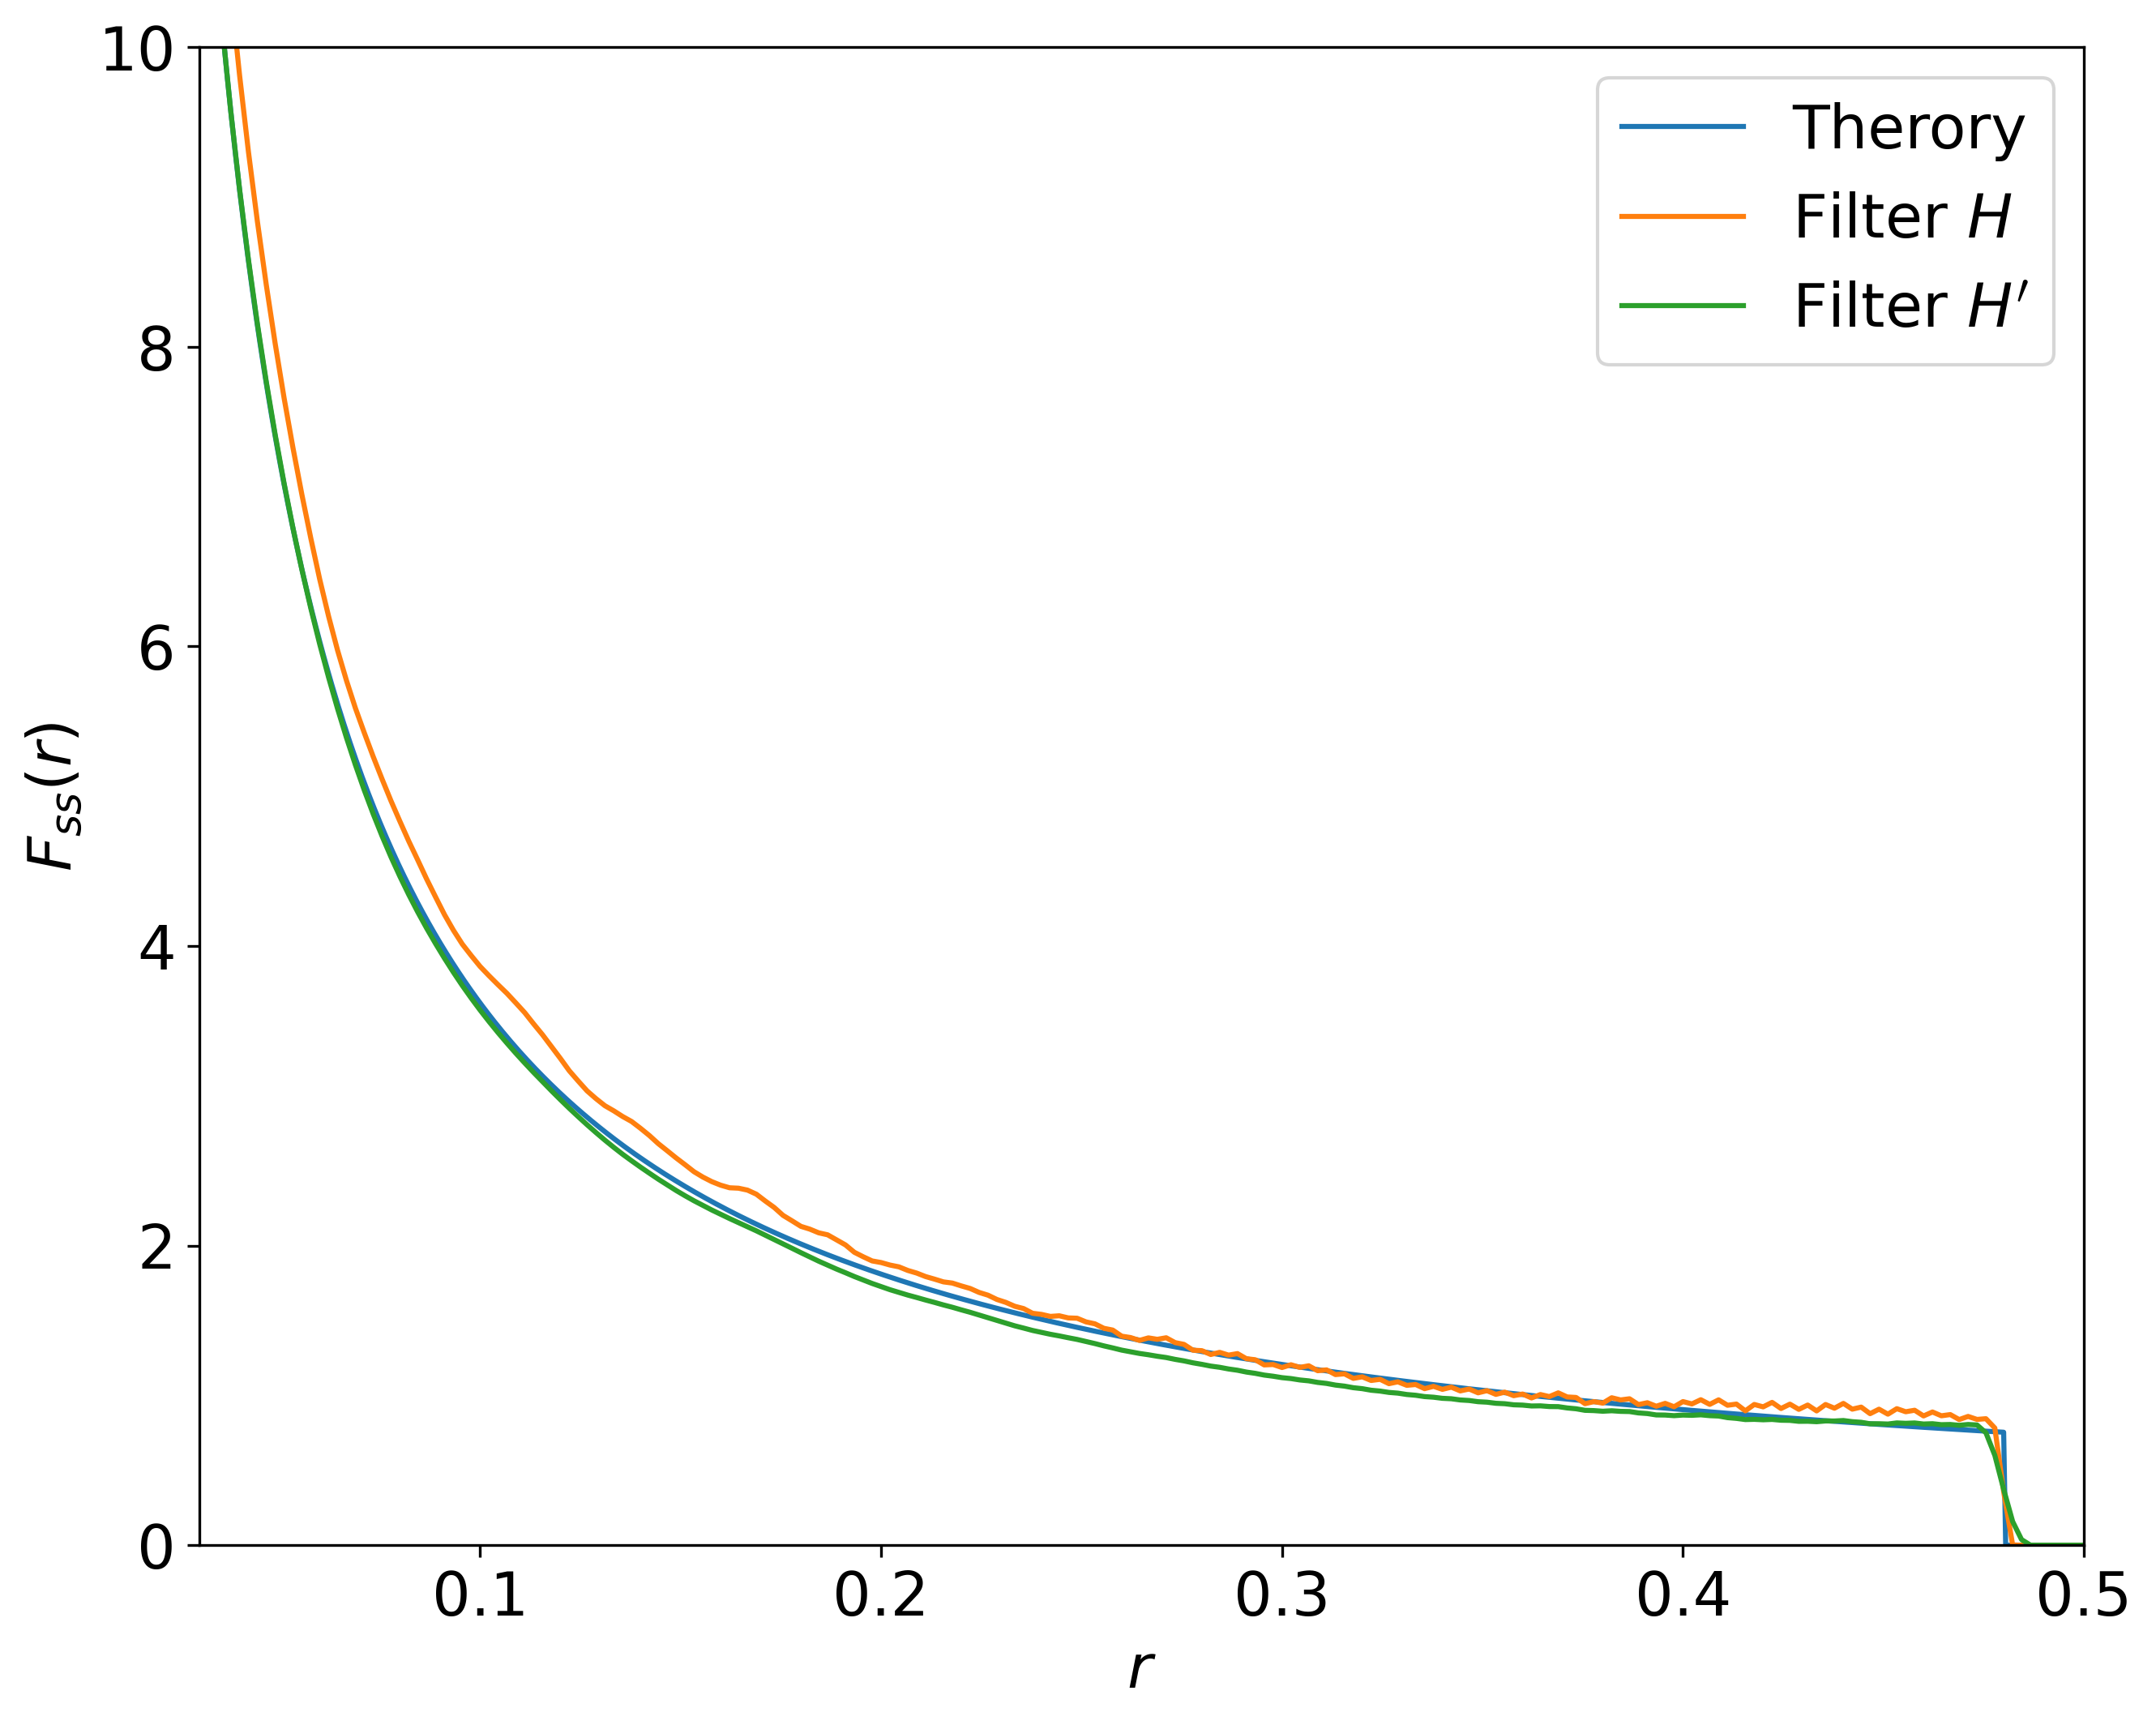
\includegraphics[width=\linewidth]{images/ball-3d-ss.png}
  \caption[]{Surface-surface function calculated for a three-dimensional ball
    with radius $R = 0.24$ using filters $H$ and $H'$. Theoretical curve is
    provided for a comparison. Image dimensions are $450 \times 450 \times 450$.}
  \label{fig:fss-ball}
\end{figure}
With the new filter calculation of $F_{ss}$ becomes more precise, even for
three-dimensional images. This can be seen in comparison with theoretical values
for known cases like the one of a ball. On \cref{fig:fss-ball} there are plots
of $F_{ss}$ function calculated with filters $H$ and $H'$ along with a
theoretical curve. It can be verified that filter $H'$ is better indeed by
calculating
\begin{equation*}
  error = \sqrt{\frac{\sum_i (F_{ss}^{calc}(x_i) -
      F_{ss}^{theory}(x_i))^2}{\sum_i F_{ss}^{theory}(x_i)^2}}
\end{equation*}
where $x_i$ belong to a set
$(\epsilon, 2R - \epsilon) \cup (2R + \epsilon, 1)$ (here we assume image
dimensions to be $1 \times 1 \times 1$ length units). Taking
$\epsilon = 0.01$ we get $error = 0.006$ for filter $H$ and $error = 0.00017$
for filter $H'$.

Unfortunately the filter $H'$ has some drawbacks in comparison with $H$. Firstly
$H$ has faster convergence with increase of image resolution. Our
acceptance criterion developed in \textcolor{red}{cite our paper again} works
also for $H'$, but sometimes it's possible to calculate a poor estimate of
$F_{ss}$ using $H$ but not $H'$. Secondly, $H'$ behaves worse that $H$ in points
of discontinuity of $F_{ss}$ as can be seen on \cref{fig:fss-disk}.

\section{Conclusion}
In this paper we develop an algorithm for precise calculation of surface-surface
correlation function for two-dimensional sets with smooth boundary and checked
our fast algorithm using these new cases. The fast algorithm was improved using
a wider filter $H'$.

\end{document}
